% =============================================================================
% Proyecto de Aula · Estadística para Ingeniería · Universidad de Medellín 2026-2
% Compilar dos veces con XeLaTeX:   xelatex informe.tex
% Todos los números provienen de valores.tex (scripts/generar_informe.py).
% =============================================================================
\documentclass[11pt]{article}
% =============================================================================
% estilo.tex — Identidad visual del informe ("papel y tinta", igual que la app)
% =============================================================================
\usepackage[letterpaper,top=2.5cm,bottom=2.5cm,left=2.6cm,right=2.4cm,headheight=14pt]{geometry}
\usepackage{mathpazo}                 % matemáticas Palatino (antes de fontspec)
\usepackage[no-math]{fontspec}
\usepackage{babel}
\babelprovide[import,main]{spanish}
\setlocalecaption{spanish}{table}{Tabla}
\setlocalecaption{spanish}{contents}{Contenido}
\setmainfont{TeX Gyre Pagella}
\newfontfamily\titular{Fraunces Proj}[UprightFont=* SemiBold,BoldFont=* Black,ItalicFont=* Italic,
  BoldItalicFont=* Bold Italic]
\newfontfamily\titularfino{Fraunces Proj}[UprightFont=* Regular,ItalicFont=* Italic]
\newfontfamily\sans{Manrope Proj}[UprightFont=* Regular,BoldFont=* Bold]
\newfontfamily\sansmedio{Manrope Proj}[UprightFont=* SemiBold,BoldFont=* ExtraBold]
\setmonofont{JetBrains Mono}[Scale=0.86]
\newfontfamily\mono{JetBrains Mono}[Scale=0.86]

\usepackage{microtype}
\usepackage{xcolor}
\definecolor{papel}{HTML}{F4EFE6}
\definecolor{tarjeta}{HTML}{FFFDF8}
\definecolor{tinta}{HTML}{1D1A16}
\definecolor{gris}{HTML}{6E665B}
\definecolor{linea}{HTML}{DCD2C1}
\definecolor{bermellon}{HTML}{D9480F}
\definecolor{oliva}{HTML}{5E7D3A}
\definecolor{pizarra}{HTML}{3E5C76}
\definecolor{crema}{HTML}{FBF4E9}
\definecolor{gristeoria}{HTML}{F0EFEA}

\usepackage{amsmath,amssymb,mathtools}
\usepackage{graphicx}
\usepackage{booktabs,tabularx,array,multirow}
\usepackage{caption,subcaption}
\usepackage{enumitem}
\usepackage{fancyhdr}
\usepackage{titlesec}
\usepackage{tikz}
\usetikzlibrary{calc,positioning,shadows}
\usepackage[most]{tcolorbox}
\usepackage{eso-pic}
\usepackage{float}
\usepackage{setspace}
\usepackage{needspace}
\usepackage[hidelinks]{hyperref}
\hypersetup{colorlinks=true,linkcolor=tinta,urlcolor=bermellon,citecolor=bermellon}
\usepackage{bookmark}

\setstretch{1.08}
\setlength{\parskip}{0.42em}
\setlength{\parindent}{0pt}
\renewcommand{\arraystretch}{1.12}
\captionsetup{font={small,sf},labelfont={bf,color=bermellon},textfont={color=tinta},labelsep=period,
  skip=4pt}
\DeclareCaptionFont{sf}{\sans}
\setlist{itemsep=2pt,topsep=3pt,leftmargin=1.3em}

% ---------- Títulos de sección ------------------------------------------------
\titleformat{\section}[block]
  {\titular\fontsize{19}{22}\selectfont\color{tinta}}
  {\color{bermellon}\titular\bfseries\fontsize{30}{30}\selectfont\thesection\hspace{10pt}}{0pt}{}
  [\vspace{-4pt}{\color{tinta}\rule{\linewidth}{1.4pt}}]
\titleformat{\subsection}{\titular\fontsize{13.2}{16}\selectfont\color{tinta}}
  {\color{bermellon}\thesubsection}{8pt}{}
\titleformat{\subsubsection}{\sansmedio\fontsize{10.4}{13}\selectfont\color{pizarra}}
  {\thesubsubsection}{6pt}{}
\titlespacing*{\section}{0pt}{10pt}{8pt}
\pretocmd{\section}{\needspace{14\baselineskip}}{}{}
\pretocmd{\subsection}{\needspace{8\baselineskip}}{}{}
\titlespacing*{\subsection}{0pt}{9pt}{3pt}
\titlespacing*{\subsubsection}{0pt}{6pt}{2pt}

% ---------- Encabezados y pies -------------------------------------------------
\pagestyle{fancy}
\fancyhf{}
\renewcommand{\headrulewidth}{0pt}
\fancyhead[L]{\mono\color{gris}\fontsize{7}{8}\selectfont ESTADÍSTICA PARA INGENIERÍA · PROYECTO DE AULA 2026-2}
\fancyhead[R]{\mono\color{gris}\fontsize{7}{8}\selectfont UNIVERSIDAD DE MEDELLÍN}
\fancyfoot[C]{\sans\color{tinta}\small\thepage}
\fancypagestyle{plain}{\fancyhf{}\fancyfoot[C]{\sans\color{tinta}\small\thepage}}

% ---------- Cajas ---------------------------------------------------------------
\newcommand{\etiquetacaja}[2]{{\mono\color{#1}\fontsize{7}{8}\selectfont #2}\par\vspace{2pt}}
\newtcolorbox{lectura}[1][]{enhanced,breakable,colback=crema,colframe=bermellon,boxrule=0pt,
  leftrule=3pt,arc=0pt,left=9pt,right=8pt,top=5pt,bottom=5pt,fontupper=\small,
  before upper=\etiquetacaja{bermellon}{LECTURA},#1}
\newtcolorbox{idea}[1][]{enhanced,breakable,colback=gristeoria,colframe=pizarra,boxrule=0pt,
  leftrule=3pt,arc=0pt,left=9pt,right=8pt,top=5pt,bottom=5pt,fontupper=\small,
  before upper=\etiquetacaja{pizarra}{#1}}
\newtcbtheorem[number within=section]{definicion}{Definición}{enhanced,breakable,colback=white,
  colframe=tinta,boxrule=0.9pt,arc=0pt,fonttitle=\sansmedio\small,coltitle=papel,colbacktitle=tinta,
  attach boxed title to top left={yshift=-2mm,xshift=3mm},boxed title style={arc=0pt,boxrule=0pt},
  top=4mm,left=6pt,right=6pt,bottom=3pt,fontupper=\small,
  drop fuzzy shadow=black!0,borderline west={3pt}{0pt}{bermellon}}{def}
\newtcbtheorem[number within=section]{teorema}{Teorema}{enhanced,breakable,colback=crema,
  colframe=bermellon,boxrule=0.9pt,arc=0pt,fonttitle=\sansmedio\small,coltitle=white,colbacktitle=bermellon,
  attach boxed title to top left={yshift=-2mm,xshift=3mm},boxed title style={arc=0pt,boxrule=0pt},
  top=4mm,left=6pt,right=6pt,bottom=3pt,fontupper=\small\itshape}{teo}
\newtcolorbox{algoritmo}[1]{enhanced,breakable,colback=white,colframe=pizarra,boxrule=0.8pt,arc=0pt,
  fonttitle=\sansmedio\small,coltitle=white,colbacktitle=pizarra,title={#1},left=6pt,right=6pt,
  fontupper=\small}

% ---------- Utilidades -----------------------------------------------------------
\newcommand{\etiqueta}[1]{{\mono\color{bermellon}\fontsize{7.5}{9}\selectfont\MakeUppercase{#1}}}
\newcommand{\rechaza}{\colorbox{bermellon}{\color{white}\sansmedio\footnotesize\,SE RECHAZA $H_0$\,}}
\newcommand{\norechaza}{\colorbox{oliva}{\color{white}\sansmedio\footnotesize\,NO SE RECHAZA $H_0$\,}}
\newcommand{\figura}[3][0.98]{\begin{figure}[H]\centering\includegraphics[width=#1\linewidth]{../figuras/#2.pdf}
  \caption{#3}\label{fig:#2}\end{figure}}
\newcommand{\tabla}[3][\small]{\begin{table}[H]\centering\caption{#3}\label{tab:#2}{#1\sans
  \input{tablas/#2.tex}}\end{table}}
\newcommand{\pyval}[1]{#1}

% Archivo generado por scripts/generar_informe.py — NO editar a mano
\newcommand{\afCrit}{1.9600}
\newcommand{\afP}{0.4037}
\newcommand{\afPmen}{0.7982}
\newcommand{\afZ}{0.8351}
\newcommand{\anAdP}{0.897}
\newcommand{\anChi}{1.003}
\newcommand{\anChiP}{0.606}
\newcommand{\anChiV}{2}
\newcommand{\anCp}{1.655}
\newcommand{\anCpk}{1.616}
\newcommand{\anIcLi}{73.9994}
\newcommand{\anIcLs}{74.0030}
\newcommand{\anKsP}{0.913}
\newcommand{\anMu}{74.00118}
\newcommand{\anPpm}{0.8}
\newcommand{\anS}{0.01007}
\newcommand{\anTn}{1.306}
\newcommand{\anTnP}{0.194}
\newcommand{\arBcero}{1.2610}
\newcommand{\arBuno}{0.7713}
\newcommand{\arDoble}{1.71}
\newcommand{\arR}{0.080}
\newcommand{\arRdos}{0.373}
\newcommand{\arRho}{0.645}
\newcommand{\arRlog}{0.611}
\newcommand{\asimA}{0.58}
\newcommand{\asimB}{0.15}
\newcommand{\asimC}{2.18}
\newcommand{\asimD}{1.26}
\newcommand{\astonEP}{6.38393}
\newcommand{\astonP}{0.4957}
\newcommand{\bnCrit}{19.675}
\newcommand{\bnEP}{14.09}
\newcommand{\bnP}{0.2278}
\newcommand{\bnPp}{0.397}
\newcommand{\bnR}{2.697}
\newcommand{\bnV}{11}
\newcommand{\cfMc}{32}
\newcommand{\cfMf}{160}
\newcommand{\cfNc}{538}
\newcommand{\cfNf}{535}
\newcommand{\cfP}{<\,0.0001}
\newcommand{\cfRazon}{5.0}
\newcommand{\cfSup}{73.7}
\newcommand{\cfZ}{13.44}
\newcommand{\cpkA}{0.606}
\newcommand{\cpkB}{0.876}
\newcommand{\cpkC}{0.982}
\newcommand{\cpkD}{0.740}
\newcommand{\cpkE}{0.423}
\newcommand{\cumpleA}{71.3}
\newcommand{\cumpleB}{81.3}
\newcommand{\cumpleC}{78.8}
\newcommand{\cumpleD}{71.1}
\newcommand{\cumpleE}{47.9}
\newcommand{\desvA}{29.42}
\newcommand{\desvB}{51.89}
\newcommand{\desvC}{187.04}
\newcommand{\desvD}{173.29}
\newcommand{\difDos}{3.554}
\newcommand{\difUno}{18.578}
\newcommand{\eaAd}{0.4573}
\newcommand{\eaAdMod}{0.4633}
\newcommand{\eaAdP}{0.232}
\newcommand{\eaCrit}{5.9915}
\newcommand{\eaD}{0.0852}
\newcommand{\eaEP}{4.9110}
\newcommand{\eaGalfa}{1.239}
\newcommand{\eaGbeta}{162.71}
\newcommand{\eaK}{5}
\newcommand{\eaKsP}{0.358}
\newcommand{\eaKsPc}{0.744}
\newcommand{\eaMu}{181.946}
\newcommand{\eaP}{0.0858}
\newcommand{\eaS}{29.415}
\newcommand{\eaV}{2}
\newcommand{\ebAd}{1.990}
\newcommand{\ebAdP}{0.0010}
\newcommand{\ebD}{0.1682}
\newcommand{\ebGAdP}{0.817}
\newcommand{\ebGalfa}{1.115}
\newcommand{\ebGbeta}{177.51}
\newcommand{\ebKsP}{0.0010}
\newcommand{\eeDos}{32.9170}
\newcommand{\eeUno}{7.7008}
\newcommand{\fCrit}{1.1541}
\newcommand{\fDen}{0.004101}
\newcommand{\fF}{2.2829}
\newcommand{\fGlDos}{734}
\newcommand{\fGlUno}{767}
\newcommand{\fIcLi}{1.978}
\newcommand{\fIcLs}{2.634}
\newcommand{\fNum}{0.009362}
\newcommand{\fP}{<\,0.0001}
\newcommand{\faF}{1.519}
\newcommand{\faFP}{0.040}
\newcommand{\faIcLi}{3.1}
\newcommand{\faIcLs}{9.8}
\newcommand{\faMdos}{74.0077}
\newcommand{\faMicras}{6.5}
\newcommand{\faMuno}{74.0012}
\newcommand{\faP}{0.0002}
\newcommand{\faT}{-3.827}
\newcommand{\feDos}{1.165}
\newcommand{\feUno}{3.112}
\newcommand{\fepDos}{0.5595}
\newcommand{\fepUno}{<\,0.0001}
\newcommand{\juBp}{0.2150}
\newcommand{\juCrit}{5.9915}
\newcommand{\juEP}{3.0760}
\newcommand{\juIcLi}{7.6}
\newcommand{\juIcLs}{13.2}
\newcommand{\juK}{4}
\newcommand{\juLic}{0.0407}
\newcommand{\juLsc}{0.3893}
\newcommand{\juP}{0.2148}
\newcommand{\juPbar}{0.2150}
\newcommand{\juPdos}{0.1108}
\newcommand{\juPz}{<\,0.0001}
\newcommand{\juV}{2}
\newcommand{\juZ}{7.101}
\newcommand{\kwH}{298.8}
\newcommand{\kwP}{<\,0.0001}
\newcommand{\levP}{<\,0.0001}
\newcommand{\levW}{111.19}
\newcommand{\lgAd}{7.071}
\newcommand{\lgAdP}{0.0020}
\newcommand{\lgChi}{86.44}
\newcommand{\lgChiP}{<\,0.0001}
\newcommand{\lgChiV}{9}
\newcommand{\lgD}{0.0466}
\newcommand{\lgKsP}{0.0020}
\newcommand{\lgMu}{4.284}
\newcommand{\lgPeq}{264}
\newcommand{\lgPeqE}{186.5}
\newcommand{\lgSig}{1.791}
\newcommand{\liClasico}{0.0}
\newcommand{\liConocido}{4.7}
\newcommand{\liDreal}{0.1130}
\newcommand{\liDtabla}{0.1723}
\newcommand{\licx}{73.98804}
\newcommand{\llDisp}{2.517}
\newcommand{\llMedia}{4.0899}
\newcommand{\llVar}{10.2927}
\newcommand{\lscr}{0.04811}
\newcommand{\lscx}{74.01431}
\newcommand{\mcMwCtrl}{5.5}
\newcommand{\mcMwDos}{6.6}
\newcommand{\mcMwUno}{10.3}
\newcommand{\mcSupCtrl}{0.500}
\newcommand{\mcSupDos}{0.522}
\newcommand{\mcSupUno}{0.534}
\newcommand{\mcTCtrl}{5.4}
\newcommand{\mcTDos}{5.1}
\newcommand{\mcTUno}{10.2}
\newcommand{\mcZCtrl}{5.7}
\newcommand{\mcZDos}{5.3}
\newcommand{\mcZUno}{10.7}
\newcommand{\medADos}{167.64}
\newcommand{\medAUno}{180.04}
\newcommand{\medBDos}{134.59}
\newcommand{\medBUno}{165.26}
\newcommand{\medPpmA}{317.4}
\newcommand{\medPpmB}{262.8}
\newcommand{\medPpmC}{289.7}
\newcommand{\medPpmD}{319.6}
\newcommand{\medPpmE}{412.8}
\newcommand{\mediaA}{181.95}
\newcommand{\mediaB}{163.37}
\newcommand{\mediaC}{201.52}
\newcommand{\mediaD}{197.97}
\newcommand{\mejor}{Marca 2}
\newcommand{\muE}{0.0062}
\newcommand{\muLi}{2.6959}
\newcommand{\muLs}{2.7083}
\newcommand{\muMedia}{2.7021}
\newcommand{\muS}{0.0829}
\newcommand{\muT}{1.9634}
\newcommand{\mwMuDos}{1\,800}
\newcommand{\mwMuUno}{1\,800}
\newcommand{\mwPDos}{0.8852}
\newcommand{\mwPUno}{0.0247}
\newcommand{\mwPpmP}{<\,0.0001}
\newcommand{\mwPpmZ}{-5.393}
\newcommand{\mwPsDos}{0.8873}
\newcommand{\mwPsUno}{0.0248}
\newcommand{\mwRDos}{3\,657.5}
\newcommand{\mwRUno}{4\,058.0}
\newcommand{\mwSigDos}{190.525}
\newcommand{\mwSigUno}{190.526}
\newcommand{\mwSupDos}{0.508}
\newcommand{\mwSupUno}{0.619}
\newcommand{\mwUDos}{1\,827.5}
\newcommand{\mwUUno}{2\,228.0}
\newcommand{\mwZDos}{0.1443}
\newcommand{\mwZUno}{2.2464}
\newcommand{\nAutores}{115}
\newcommand{\nCommits}{2\,238}
\newcommand{\nDias}{523}
\newcommand{\nHornos}{3\,665}
\newcommand{\nMarcaA}{812}
\newcommand{\nMarcaB}{694}
\newcommand{\nMarcaC}{735}
\newcommand{\nMarcaD}{768}
\newcommand{\nMarcaE}{656}
\newcommand{\nMejor}{694}
\newcommand{\normAdCuatro}{0.230}
\newcommand{\normAdTres}{0.843}
\newcommand{\normKsCuatro}{0.129}
\newcommand{\normKsTres}{0.718}
\newcommand{\normMejorAd}{0.653}
\newcommand{\normMejorAdP}{0.091}
\newcommand{\normMejorChi}{9.314}
\newcommand{\normMejorChiP}{0.231}
\newcommand{\normMejorKsD}{0.0292}
\newcommand{\normMejorKsP}{0.168}
\newcommand{\normMejorV}{7}
\newcommand{\pcDos}{26.3}
\newcommand{\pcLi}{22.3}
\newcommand{\pcLs}{25.8}
\newcommand{\pcNdos}{1\,371}
\newcommand{\pcNuno}{867}
\newcommand{\pcP}{0.0020}
\newcommand{\pcTot}{24.0}
\newcommand{\pcUno}{20.5}
\newcommand{\pcZ}{-3.089}
\newcommand{\pctCumpleTotal}{70.5}
\newcommand{\pnBn}{10}
\newcommand{\pnPoi}{8}
\newcommand{\pnReal}{10}
\newcommand{\poiCCrit}{15.507}
\newcommand{\poiCEP}{334.08}
\newcommand{\poiCP}{<\,0.0001}
\newcommand{\poiCV}{8}
\newcommand{\poiCeros}{50}
\newcommand{\poiCerosE}{8.8}
\newcommand{\poiEP}{0.0814}
\newcommand{\poiLam}{0.3141}
\newcommand{\poiP}{0.7755}
\newcommand{\poiV}{1}
\newcommand{\potDentroA}{94.83}
\newcommand{\potDentroB}{99.71}
\newcommand{\potDentroC}{100.00}
\newcommand{\potDentroD}{98.05}
\newcommand{\potDentroE}{89.02}
\newcommand{\potMediaA}{2.6685}
\newcommand{\potMediaB}{2.7021}
\newcommand{\potMediaC}{2.7314}
\newcommand{\potMediaD}{2.7051}
\newcommand{\potMediaE}{2.6250}
\newcommand{\potSA}{0.1036}
\newcommand{\potSB}{0.0829}
\newcommand{\potSC}{0.0640}
\newcommand{\potSD}{0.0968}
\newcommand{\potSE}{0.1142}
\newcommand{\prE}{0.0290}
\newcommand{\prLi}{0.7837}
\newcommand{\prLs}{0.8417}
\newcommand{\prP}{0.8127}
\newcommand{\prWLi}{0.7820}
\newcommand{\prWLs}{0.8400}
\newcommand{\prX}{564}
\newcommand{\rRepPpm}{0.272}
\newcommand{\rUsoPot}{-0.137}
\newcommand{\rUsoPpm}{0.307}
\newcommand{\rUsoRep}{0.432}
\newcommand{\razonS}{1.51}
\newcommand{\rb}{0.02276}
\newcommand{\regBcero}{5.5219}
\newcommand{\regBuno}{0.0466}
\newcommand{\regPct}{4.77}
\newcommand{\regRdos}{0.093}
\newcommand{\repAnioMejor}{0.068}
\newcommand{\repAnioPeor}{0.205}
\newcommand{\sCuatro}{0.0968}
\newcommand{\sLi}{0.0788}
\newcommand{\sLs}{0.0875}
\newcommand{\sTres}{0.0640}
\newcommand{\segunda}{Marca 3}
\newcommand{\sobreNormaA}{0.74}
\newcommand{\sobreNormaB}{0.00}
\newcommand{\sobreNormaC}{0.14}
\newcommand{\sobreNormaD}{0.65}
\newcommand{\sobreNormaE}{3.66}
\newcommand{\sumaMejor}{7}
\newcommand{\sumaSegunda}{8}
\newcommand{\tamMax}{50\,726}
\newcommand{\tamMed}{87}
\newcommand{\tamMedia}{294}
\newcommand{\tamPnov}{677}
\newcommand{\tcritDos}{1.9803}
\newcommand{\tcritUno}{1.9857}
\newcommand{\tglDos}{118}
\newcommand{\tglUno}{93.37}
\newcommand{\tpDos}{0.9142}
\newcommand{\tpUno}{0.0178}
\newcommand{\ttDos}{0.1080}
\newcommand{\ttUno}{2.4125}
\newcommand{\ttipoDos}{combinada}
\newcommand{\ttipoUno}{Welch}
\newcommand{\usoProm}{4.97}
\newcommand{\vaChiDer}{767.84}
\newcommand{\vaChiIzq}{621.94}
\newcommand{\vaLi}{0.006204}
\newcommand{\vaLs}{0.007659}
\newcommand{\vaSdos}{0.006874}
\newcommand{\xbb}{74.00118}
\newcommand{\zpDos}{0.9140}
\newcommand{\zpUno}{0.0158}
\newcommand{\zzDos}{0.1080}
\newcommand{\zzUno}{2.4125}


\title{Decidir con datos: de los hornos al código}
\author{Juan Manuel Moreno Muñoz \and David Restrepo \and Juan Fernando}
\hypersetup{pdftitle={Proyecto de Aula · Estadística para Ingeniería},
  pdfauthor={Juan Manuel Moreno Muñoz, David Restrepo, Juan Fernando}}

\begin{document}
% =============================================================================
% PORTADA
% =============================================================================
\begin{titlepage}
\AddToShipoutPictureBG*{\AtPageLowerLeft{\color{papel}\rule{\paperwidth}{\paperheight}}}
\begin{tikzpicture}[remember picture,overlay]
  % trama de puntos
  \foreach \i in {0,...,44} \foreach \j in {0,...,57}
    {\fill[tinta!9] ($(current page.south west)+(\i*0.5cm,\j*0.5cm)$) circle (0.45pt);}
  \fill[bermellon] ($(current page.north west)+(0,-0.9cm)$) rectangle ($(current page.north east)+(0,-1.15cm)$);
  \node[anchor=north west,inner sep=0] at ($(current page.north west)+(2.6cm,-1.9cm)$)
    {\mono\color{tinta}\fontsize{8.5}{10}\selectfont FACULTAD DE INGENIERÍAS · UNIVERSIDAD DE MEDELLÍN};
  \node[anchor=north east,inner sep=0] at ($(current page.north east)+(-2.4cm,-1.9cm)$)
    {\mono\color{tinta}\fontsize{8.5}{10}\selectfont 2026-2};
  % gran numeral de fondo
  \node[anchor=south east,inner sep=0] at ($(current page.south east)+(-1.2cm,2.2cm)$)
    {\titular\bfseries\fontsize{230}{230}\selectfont\color{bermellon!12}$\chi^2$};
\end{tikzpicture}
\vspace*{3.4cm}
{\mono\color{bermellon}\fontsize{10}{12}\selectfont ESTADÍSTICA PARA INGENIERÍA · PROYECTO DE AULA\par}
\vspace{0.6cm}
{\titular\bfseries\fontsize{50}{50}\selectfont\color{tinta} Decidir\\[2pt] con {\titularfino\itshape\color{bermellon}datos}:\par}
\vspace{0.25cm}
{\titular\fontsize{25}{29}\selectfont\color{tinta} de los hornos al código\par}
\vspace{0.7cm}
{\color{tinta}\rule{4cm}{2pt}\par}
\vspace{0.5cm}
\begin{minipage}{0.84\textwidth}
{\sans\fontsize{11.5}{17}\selectfont\color{tinta!85}Pruebas de bondad de ajuste ($\chi^2$, Kolmogorov–Smirnov y
Anderson–Darling), intervalos de confianza y pruebas de hipótesis aplicados a un estudio de mercado de hornos a
gas, a la comparación de dos equipos de procesamiento y a dos casos con datos \textbf{reales} de Ingeniería de
Sistemas e Ingeniería Industrial, con una herramienta propia en Python.\par}
\end{minipage}
\vfill
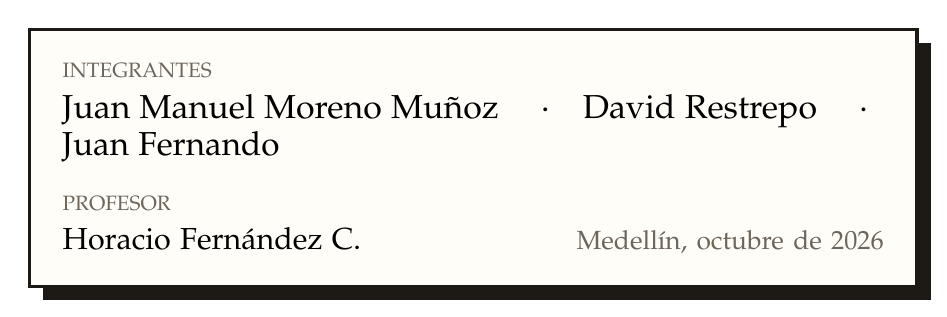
\begin{tikzpicture}
\node[draw=tinta,line width=1.3pt,fill=tarjeta,inner sep=12pt,text width=0.86\textwidth,
      drop shadow={shadow xshift=5pt,shadow yshift=-5pt,fill=tinta,opacity=1}] {
  {\mono\color{gris}\fontsize{7.5}{9}\selectfont INTEGRANTES}\par\vspace{3pt}
  {\sansmedio\fontsize{12}{16}\selectfont Juan Manuel Moreno Muñoz \quad·\quad David Restrepo \quad·\quad Juan Fernando}\par
  \vspace{8pt}
  {\mono\color{gris}\fontsize{7.5}{9}\selectfont PROFESOR}\par\vspace{2pt}
  {\sans\fontsize{11}{14}\selectfont Horacio Fernández C.}\hfill
  {\sans\fontsize{9.5}{12}\selectfont\color{gris} Medellín, octubre de 2026}
};
\end{tikzpicture}
\vspace*{0.6cm}
\end{titlepage}

% =============================================================================
% RESUMEN E ÍNDICE
% =============================================================================
\pagenumbering{roman}
\setcounter{page}{2}
\section*{Resumen}
Este proyecto aplica las herramientas de la Estadística para Ingeniería a la toma de decisiones en tres
problemas. En el \textbf{primero}, con una base de \nHornos{} hornos de cinco marcas, se comparan las emisiones y la
potencia, se elige la marca de mejor desempeño (\mejor) y se construyen intervalos de confianza para su media, su
varianza y su proporción de cumplimiento; además se contrastan la variabilidad de dos tecnologías y la afirmación
de un fabricante. En el \textbf{segundo}, con datos simulados, se comparan dos equipos de procesamiento mediante
pruebas de bondad de ajuste, pruebas $t$ y $Z$ y la prueba no paramétrica de Mann–Whitney, y se mide la potencia
de cada prueba con un estudio de Monte Carlo. En el \textbf{tercero} se analizan datos reales: el historial de
\nCommits{} commits del proyecto de código abierto Streamlit (Ingeniería de Sistemas) y dos bases clásicas de
control de calidad (Ingeniería Industrial). Como valor agregado se explican y aplican las pruebas de
Kolmogorov–Smirnov y Anderson–Darling, con valores $p$ corregidos por simulación cuando los parámetros se estiman,
y se entrega una aplicación web que permite repetir todo el análisis con cualquier archivo de datos.

{\sloppy\textbf{Palabras clave:} bondad de ajuste, Kolmogorov–Smirnov, Anderson–Darling, Mann–Whitney, intervalos de
confianza, control estadístico de procesos, binomial negativa.\par}

\newpage
{\small\sans\setstretch{1.05}\tableofcontents}

% =============================================================================
\newpage
\pagenumbering{arabic}
\section*{Introducción}
\addcontentsline{toc}{section}{Introducción}
En ingeniería casi ninguna decisión se toma con certeza: el horno que se compra, el servidor que se dimensiona o
la máquina que se ajusta se eligen a partir de muestras, y las muestras varían. La Estadística ofrece el lenguaje
para cuantificar esa incertidumbre y decidir con un riesgo conocido. Este informe reúne los temas del curso
—estadística descriptiva, distribuciones de probabilidad, estimación, intervalos de confianza, pruebas de hipótesis
y bondad de ajuste— y los aplica a tres problemas, siguiendo el enunciado del proyecto de aula.

Un hilo conductor atraviesa todo el trabajo: \emph{casi todos los métodos inferenciales suponen un modelo} (que
los datos sean normales, que los conteos sean Poisson o binomiales). Por eso las pruebas de bondad de ajuste no
son un tema aislado: son el paso que valida los demás. La guía del curso presenta la prueba $\chi^2$
\cite{guia}; como valor agregado se estudian a fondo las pruebas de Kolmogorov–Smirnov (KS) y Anderson–Darling
(AD), que no necesitan agrupar los datos y son más potentes \cite{stephens,razali}.

El documento se organiza así: la sección~\ref{sec:marco} presenta el marco teórico; las secciones
\ref{sec:p1}, \ref{sec:p2} y \ref{sec:p3} desarrollan los tres puntos del enunciado; al final se presentan las
conclusiones y, en los anexos, la herramienta construida, la solución del taller de la guía y la equivalencia de
los cálculos en Excel y R. Para garantizar la reproducibilidad, todos los números del informe se generan con el
código del repositorio (semilla 2026) y ninguno se copió a mano.

\begin{idea}{HERRAMIENTA}
La aplicación web (Python + Streamlit) incluye cada punto con sus gráficas interactivas, un laboratorio para
subir \emph{cualquier} archivo (CSV, Excel, TXT, JSON) y aplicarle todas las pruebas, la teoría de las tres pruebas
de ajuste con simulaciones y la guía de bondad de ajuste resuelta. Véase el anexo~\ref{anx:app}.
\end{idea}

% =============================================================================
\newpage
\section{Marco teórico}\label{sec:marco}
% =============================================================================
\subsection{Estimación e intervalos de confianza}
Un estimador es una función de la muestra que aproxima un parámetro. En el proyecto se usan los estimadores de
\textbf{máxima verosimilitud} (MV): $\hat\theta=\arg\max_\theta\prod_{i=1}^n f(x_i;\theta)$. Para la Poisson
$\hat\lambda=\bar x$; para la binomial $\hat p=\bar x/n$; para la gamma (forma $\alpha$, escala $\beta$) y la
lognormal las ecuaciones se resuelven numéricamente. Los intervalos utilizados son \cite{walpole,montgomery}:
\begin{equation}
\bar x\pm t_{\alpha/2,\,n-1}\frac{s}{\sqrt n},\qquad
\frac{(n-1)s^2}{\chi^2_{\alpha/2,\,n-1}}\le\sigma^2\le\frac{(n-1)s^2}{\chi^2_{1-\alpha/2,\,n-1}},\qquad
\hat p\pm z_{\alpha/2}\sqrt{\frac{\hat p(1-\hat p)}{n}},
\label{eq:ic}
\end{equation}
donde $\chi^2_{a,v}$ deja un área $a$ a su derecha. El de la media es válido para $n$ grande aunque los datos no
sean normales (Teorema del Límite Central); el de la varianza \emph{exige normalidad}, y por eso se verifica antes
con pruebas de ajuste.

\subsection{Pruebas de hipótesis}
Se plantea $H_0$ y se calcula un estadístico cuya distribución es conocida cuando $H_0$ es cierta; se rechaza
$H_0$ si el valor $P$ es menor que el nivel de significancia $\alpha$ (aquí $0.05$). La tabla~\ref{tab:pruebas}
resume los estadísticos del proyecto.
\begin{table}[H]\centering\small\caption{Estadísticos de prueba utilizados.}\label{tab:pruebas}
\begin{tabular}{lll}\toprule
\textbf{Hipótesis nula} & \textbf{Estadístico} & \textbf{Distribución bajo $H_0$}\\\midrule
$\sigma_1^2=\sigma_2^2$ & $F=s_1^2/s_2^2$ & $F_{(n_1-1,\,n_2-1)}$\\[2pt]
$\mu_1=\mu_2$ ($\sigma^2$ iguales) & $t=\dfrac{\bar x_1-\bar x_2}{s_p\sqrt{1/n_1+1/n_2}}$ & $t_{(n_1+n_2-2)}$\\[8pt]
$\mu_1=\mu_2$ ($\sigma^2$ distintas, Welch) & $t=\dfrac{\bar x_1-\bar x_2}{\sqrt{s_1^2/n_1+s_2^2/n_2}}$ &
$t_{(v)}$, $v$ de Satterthwaite\\[8pt]
$\mu_1=\mu_2$ ($n$ grande) & $Z=\dfrac{\bar x_1-\bar x_2}{\sqrt{s_1^2/n_1+s_2^2/n_2}}$ & $N(0,1)$ por el TLC\\[8pt]
$p=p_0$ & $Z=\dfrac{\hat p-p_0}{\sqrt{p_0(1-p_0)/n}}$ & $N(0,1)$\\\bottomrule
\end{tabular}\end{table}

\subsection{Pruebas de bondad de ajuste}\label{sec:gof}
Contrastan $H_0$: \emph{la muestra proviene de la distribución $F_0$} contra $H_a$: \emph{no proviene de $F_0$}
\cite{guia}. Las tres pruebas del proyecto miden la discrepancia entre los datos y $F_0$ de forma distinta.

\begin{definicion}{Prueba $\chi^2$ de Pearson}{chi}
Se agrupan los $n$ datos en $k$ clases con frecuencias observadas $O_i$. Si $P_i$ es la probabilidad de la clase
$i$ bajo $F_0$ y $E_i=nP_i$, el estadístico
\[EP=\sum_{i=1}^{k}\frac{(O_i-E_i)^2}{E_i}\ \sim\ \chi^2_{(v)},\qquad v=k-p-1,\]
donde $p$ es el número de parámetros estimados con la muestra. Se rechaza $H_0$ si $EP>\chi^2_{(\alpha,v)}$. Se
exige $E_i\ge5$, agrupando clases adyacentes si es necesario, y $k$ es el menor entero con $2^k>n$.
\end{definicion}
Es la única de las tres que sirve para variables \emph{discretas}. Su debilidad es que al agrupar pierde
información y que el resultado depende de las clases. Con datos muy asimétricos, las clases de igual ancho dejan
casi todo en la primera clase y, tras agrupar, quedan pocos grados de libertad; por eso también se usa la variante
con \textbf{clases equiprobables} ($P_i=1/k$ para todas, de modo que $E_i=n/k$).

\begin{definicion}{Función de distribución empírica y estadístico de Kolmogorov–Smirnov}{ks}
Con la muestra ordenada $x_{(1)}\le\dots\le x_{(n)}$, la función empírica es $F_n(x)=\#\{x_i\le x\}/n$, una escalera
que sube $1/n$ en cada dato. El estadístico KS es la mayor distancia vertical entre $F_n$ y $F_0$
\cite{kolmogorov,smirnov}:
\[D=\sup_x\left|F_n(x)-F_0(x)\right|=\max(D^+,D^-),\quad
D^+=\max_i\Big(\tfrac{i}{n}-F_0(x_{(i)})\Big),\quad D^-=\max_i\Big(F_0(x_{(i)})-\tfrac{i-1}{n}\Big).\]
\end{definicion}
\begin{teorema}{Glivenko–Cantelli y distribución de Kolmogorov}{gc}
Si $H_0$ es cierta, $D\to0$ con probabilidad 1 cuando $n\to\infty$. Si además $F_0$ es continua y está
completamente especificada, la distribución de $D$ no depende de $F_0$ y
$P(\sqrt n\,D>t)\to2\sum_{j\ge1}(-1)^{j-1}e^{-2j^2t^2}$; al 5\,\% el valor crítico es aproximadamente $1.36/\sqrt n$.
\end{teorema}

\begin{figure}[H]\centering
\begin{subfigure}{0.49\linewidth}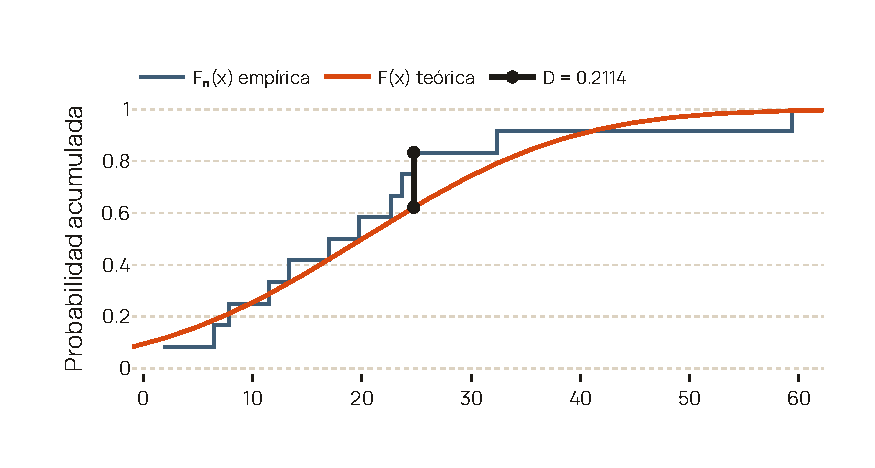
\includegraphics[width=\linewidth]{../figuras/f_ks_concepto.pdf}
\caption{KS: la mayor distancia vertical $D$.}\end{subfigure}\hfill
\begin{subfigure}{0.49\linewidth}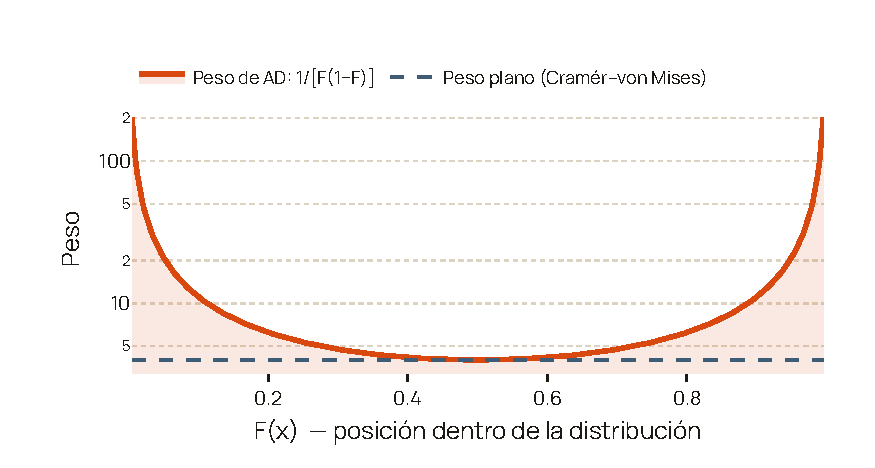
\includegraphics[width=\linewidth]{../figuras/f_peso_ad.pdf}
\caption{AD: peso $1/[F(1-F)]$ en escala logarítmica.}\end{subfigure}
\caption{Cómo miden la discrepancia las pruebas KS y AD.}\label{fig:ksad}
\end{figure}

\begin{definicion}{Estadístico de Anderson–Darling}{ad}
Anderson y Darling \cite{ad1952,ad1954} proponen sumar las diferencias al cuadrado en todo el rango, ponderadas
por $\psi(F)=1/[F(1-F)]$:
\[A^2=n\int_{-\infty}^{\infty}\frac{[F_n(x)-F_0(x)]^2}{F_0(x)[1-F_0(x)]}\,dF_0(x)
=-n-\frac1n\sum_{i=1}^{n}(2i-1)\Big[\ln F_0(x_{(i)})+\ln\big(1-F_0(x_{(n+1-i)})\big)\Big].\]
\end{definicion}
El peso vale 4 en la mediana y crece sin límite cuando $F\to0$ o $F\to1$ (figura~\ref{fig:ksad}b): una misma
diferencia pesa mucho más en las \textbf{colas}. En ingeniería las colas son justamente lo importante (el horno que
más contamina, el tiempo de respuesta más lento), y por eso AD es la más potente de las tres. Sus valores críticos
dependen de $F_0$: para la normal con $\mu$ y $\sigma$ estimadas, Stephens \cite{stephens} usa
$A^*=A^2(1+0.75/n+2.25/n^2)$ con crítico $0.752$ al 5\,\%; con parámetros conocidos el crítico es $2.492$.

\subsubsection{El problema de estimar los parámetros: Lilliefors y el bootstrap paramétrico}
El teorema~\ref{teo:gc} supone $F_0$ \emph{conocida}. Si sus parámetros se estiman con la misma muestra, el modelo
``se acomoda'' a los datos y $D$ sale más pequeño, así que la tabla de Kolmogorov ya no sirve \cite{lilliefors}.
Se verificó por simulación: con 2000 muestras normales de tamaño 60, la prueba con la tabla rechazó el
\liConocido\,\% de las veces cuando $\mu,\sigma$ eran conocidas (correcto, $\approx\alpha$), pero solo el
\liClasico\,\% cuando se estimaban; el crítico real es \liDreal{} y no \liDtabla. Por eso, en todo el proyecto los
valores $P$ de KS y AD se obtienen por Monte Carlo:
\begin{algoritmo}{Valor $P$ por bootstrap paramétrico (corrección de Lilliefors generalizada)}
\begin{enumerate}[leftmargin=1.5em]
\item Estimar $\hat\theta$ con la muestra y calcular el estadístico observado ($D$ o $A^2$).
\item Repetir $B=999$ veces: simular $n$ datos de $F_0(\cdot;\hat\theta)$, \emph{re-estimar} $\hat\theta^*$ con
ellos y calcular el estadístico $D^*$ o $A^{2*}$.
\item Valor $P\approx(\#\{\text{estadísticos simulados}\ge\text{observado}\}+1)/(B+1)$.
\end{enumerate}
\end{algoritmo}
La tabla~\ref{tab:potencia_gof} compara, también por simulación, la \textbf{potencia} de las tres pruebas para
detectar que unos datos \emph{no} son normales ($n=60$): AD es la mejor en los tres casos y $\chi^2$ la peor, en
línea con lo reportado por Razali y Wah \cite{razali}.
\tabla{potencia_gof}{Porcentaje de veces que cada prueba rechaza la normalidad (600 réplicas, $n=60$, $\alpha=0.05$).}

\subsection{Prueba de Mann–Whitney (Wilcoxon de suma de rangos)}
Es la alternativa no paramétrica a la prueba $t$ para dos muestras independientes \cite{mannwhitney,wilcoxon}.
\begin{definicion}{Estadístico $U$ de Mann–Whitney}{mw}
Se juntan las $N=n_1+n_2$ observaciones, se ordenan y se asigna a cada una su rango (los empates reciben el rango
promedio). Si $R_1$ es la suma de rangos de la muestra 1, $U_1=R_1-n_1(n_1+1)/2$ es el número de pares
$(x_{1i},x_{2j})$ con $x_{1i}>x_{2j}$. $H_0$: ambas poblaciones son iguales, es decir, $P(X_1>X_2)=0.5$.
\end{definicion}
\begin{teorema}{Normalidad asintótica de $U$}{u}
Bajo $H_0$, $E[U]=\frac{n_1n_2}{2}$ y $Var[U]=\frac{n_1n_2}{12}\Big[(N+1)-\frac{\sum_j(t_j^3-t_j)}{N(N-1)}\Big]$
($t_j$: tamaño de cada grupo de empates); para $n_1,n_2>10$, $Z=(U_1-E[U])/\sqrt{Var[U]}\approx N(0,1)$.
\end{teorema}
Como solo usa el orden, no exige normalidad y no la afectan los atípicos; si los datos sí son normales pierde poca
potencia frente a la $t$ (eficiencia asintótica $3/\pi\approx0.955$).

\subsection{Control estadístico de procesos}
Con especificaciones $[LIE,LSE]$, los índices de capacidad son $C_p=(LSE-LIE)/6s$ y
$C_{pk}=\min(LSE-\bar x,\ \bar x-LIE)/3s$; un proceso se considera capaz si $C_{pk}\ge1.33$ \cite{montgomeryqc}.
Las cartas de control $\bar X$–$R$ usan los límites $\bar{\bar x}\pm A_2\bar R$ y $[D_3\bar R,D_4\bar R]$ (para
muestras de 5: $A_2=0.577$, $D_3=0$, $D_4=2.114$), y la carta $p$, $\bar p\pm3\sqrt{\bar p(1-\bar p)/n}$; ambas
suponen normalidad o binomialidad, que se verifican con las pruebas de ajuste.

% =============================================================================
\section{Punto 1: estudio de mercado de hornos a gas}\label{sec:p1}
% =============================================================================
La base contiene \nHornos{} hornos de cinco marcas con su tiempo de uso, número de reparaciones, emisiones (ppm) y
potencia (kW). Los datos son \textbf{inventados} pero coherentes con el enunciado: las emisiones crecen con el uso
y con las reparaciones, las reparaciones son conteos de Poisson y la potencia se degrada levemente con los años.
Especificaciones: potencia $2.7\pm0.22$ kW ($LIE=2.48$, $LSE=2.92$) y emisiones de máximo 400 ppm por seguridad
(la norma permite 1000).

\subsection*{a) Emisiones: diagrama de cajas y bigotes}
\figura[0.82]{f_cajas_ppm}{Emisiones por marca. La línea discontinua es el límite de seguridad; la punteada roja, la norma.}
\tabla[\footnotesize]{ppm}{Resumen de las emisiones (ppm) por marca.}
\begin{lectura}
Las cinco cajas son asimétricas a la derecha: bigote superior largo y atípicos solo hacia arriba, porque unos pocos
hornos (los más usados o reparados) emiten mucho más que el resto. \textbf{Marca 2 es la que menos contamina}: tiene
la caja más baja, la menor mediana (\medPpmB{} ppm), el \cumpleB\,\% de sus hornos bajo 400 ppm y ninguno sobre la
norma. Marca 5 es la peor (mediana \medPpmE{} ppm, \sobreNormaE\,\% sobre 1000 ppm). La diferencia no es casual:
Kruskal–Wallis da $H=\kwH$ ($P\kwP$) y Mann–Whitney entre las dos mejores, Marca 2 y Marca 3, da $Z=\mwPpmZ$
($P\mwPpmP$).
\end{lectura}

\subsection*{b) Cumplimiento de la especificación de potencia}
\begin{figure}[H]\centering
\begin{minipage}{0.47\linewidth}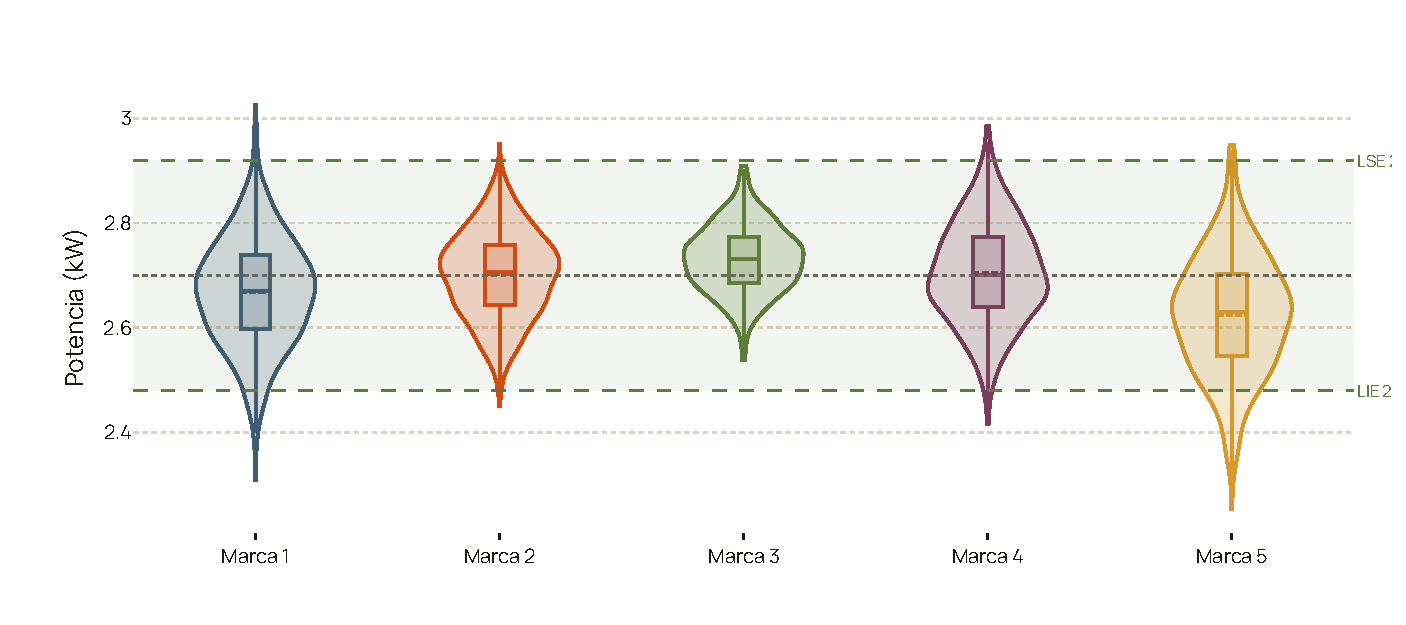
\includegraphics[width=\linewidth]{../figuras/f_potencia.pdf}\end{minipage}\hfill
\begin{minipage}{0.51\linewidth}{\footnotesize\sans\begin{tabular}{lrrrrrrr}
\toprule
\textbf{Marca} & \textbf{n} & \textbf{Media} & \textbf{Desv. (s)} & \textbf{$|\bar x-2.70|$} & \textbf{\% dentro de espec.} & \textbf{Cp} & \textbf{Cpk} \\ \midrule
Marca 1 & 812 & 2.6685 & 0.1036 & 0.0315 & 94.83 & 0.708 & 0.606 \\
Marca 2 & 694 & 2.7021 & 0.0829 & 0.0021 & 99.71 & 0.885 & 0.876 \\
Marca 3 & 735 & 2.7314 & 0.0640 & 0.0314 & 100.00 & 1.145 & 0.982 \\
Marca 4 & 768 & 2.7051 & 0.0968 & 0.0051 & 98.05 & 0.758 & 0.740 \\
Marca 5 & 656 & 2.6250 & 0.1142 & 0.0750 & 89.02 & 0.642 & 0.423 \\
\bottomrule
\end{tabular}}\end{minipage}
\caption{Potencia por marca (franja verde: especificación) e índices de capacidad.}\label{fig:pot}
\end{figure}
\begin{lectura}
La media cercana a 2.70 kW no basta; importa cuántas desviaciones caben hasta el límite más cercano, que es lo que
mide $C_{pk}$. \textbf{Marca 3 es la que mejor se ajusta} a la especificación: el mayor $C_{pk}$ (\cpkC), la menor
desviación (\potSC{} kW) y el \potDentroC\,\% de sus hornos dentro de 2.48–2.92 kW. Marca 2 está mejor centrada
($\bar x=\potMediaB$) pero es más dispersa ($C_{pk}=\cpkB$). Ninguna marca alcanza $C_{pk}\ge1.33$, y Marca 5 es la
peor ($C_{pk}=\cpkE$, \potDentroE\,\% en especificación).
\end{lectura}

\subsection*{c) Marca de mejor desempeño}
Se ordenaron las marcas (1 = mejor) en cinco criterios con igual peso; las reparaciones se dividen entre los años de
uso para no castigar a las marcas con hornos más antiguos.
\tabla[\footnotesize]{desempeno}{Criterios de desempeño y puesto de cada marca.}
\begin{lectura}
\textbf{\mejor{} tiene el mejor desempeño} (suma \sumaMejor): es la que menos contamina, la que menos se daña
(\repAnioMejor{} reparaciones por año de uso, frente a \repAnioPeor{} de Marca 5) y la segunda en potencia.
\segunda{} queda cerca (suma \sumaSegunda) gracias a su potencia más estable. Si la prioridad fuera solo la
estabilidad del quemador se elegiría \segunda; como el enunciado prioriza seguridad y desempeño global, se escoge
\mejor{}.
\end{lectura}

\subsection*{d) Intervalos de confianza del 95\,\% para \mejor}
Antes de construir el intervalo de la varianza se verificó la normalidad de la potencia: $\chi^2$: $EP=\normMejorChi$,
$v=\normMejorV$, $P=\normMejorChiP$; KS: $D=\normMejorKsD$, $P=\normMejorKsP$; AD: $A^2=\normMejorAd$,
$P=\normMejorAdP$. Ninguna prueba rechaza, así que la ecuación~\eqref{eq:ic} es aplicable ($n=\nMejor$):
\begin{align*}
\mu&:\ \muMedia\pm\muT\cdot\frac{\muS}{\sqrt{\nMejor}}=\muMedia\pm\muE
&&\Rightarrow\quad \boxed{\muLi\le\mu\le\muLs\ \text{kW}}\\
\sigma^2&:\ \frac{(\nMejor-1)\,\vaSdos}{\vaChiDer}\le\sigma^2\le\frac{(\nMejor-1)\,\vaSdos}{\vaChiIzq}
&&\Rightarrow\quad \boxed{\vaLi\le\sigma^2\le\vaLs\ \text{kW}^2}\\
p&:\ \prP\pm1.96\sqrt{\frac{\prP(1-\prP)}{\nMejor}}=\prP\pm\prE
&&\Rightarrow\quad \boxed{\prLi\le p\le\prLs}
\end{align*}
\begin{lectura}
Con 95\,\% de confianza, la potencia media de \mejor{} está entre \muLi{} y \muLs{} kW, intervalo que
\textbf{contiene el valor nominal 2.70}: el proceso está centrado. La desviación estándar está entre \sLi{} y
\sLs{} kW, y entre el \prLi{} y el \prLs{} de los hornos (\prX{} de \nMejor{} en la muestra) cumple el límite de
400 ppm (intervalo de Wilson: \prWLi–\prWLs).
\end{lectura}

\subsection*{e) Variabilidad de la potencia: Marca 3 frente a Marca 4}
$H_0:\sigma_3^2=\sigma_4^2$ contra $H_a:\sigma_3^2\ne\sigma_4^2$. La prueba $F$ supone normalidad, que se verificó
para ambas marcas (AD: $P=\normAdTres$ y $P=\normAdCuatro$).
\begin{gather*}
F=\frac{s_4^2}{s_3^2}=\frac{\fNum}{\fDen}=\fF\qquad F_{(0.025;\,\fGlUno,\,\fGlDos)}=\fCrit\qquad P\fP\\
\text{IC 95\,\% de }\sigma_4^2/\sigma_3^2:\ [\fIcLi,\ \fIcLs]
\end{gather*}
\begin{lectura}
\rechaza\quad La desviación de Marca 4 (\sCuatro{} kW) es \razonS{} veces la de Marca 3 (\sTres{} kW); el
intervalo para la razón de varianzas no contiene el 1 y la prueba de Levene, que no exige normalidad, lo confirma
($W=\levW$, $P\levP$). \textbf{Sí hay diferencia: la tecnología de Marca 3 produce una potencia más uniforme.}
\end{lectura}

\subsection*{f) ¿80 de cada 100 hornos de \mejor{} cumplen la norma de emisión?}
$H_0:p=0.80$ contra $H_a:p\ne0.80$: $Z=(\prP-0.80)/\sqrt{0.80(0.20)/\nMejor}=\afZ$, con crítico $\pm\afCrit$ y
$P=\afP$. Para la versión unilateral $H_a:p<0.80$, $P=\afPmen$.
\begin{lectura}
\norechaza\quad La proporción observada (\prP) está a solo \afZ{} errores estándar del 80\,\%, y el intervalo del
literal d) contiene 0.80. \textbf{Estamos de acuerdo con la afirmación del fabricante}: los datos son consistentes
con que 80 de cada 100 hornos cumplen.
\end{lectura}

\subsection*{Relaciones entre las variables}
\begin{figure}[H]\centering
\begin{minipage}{0.44\linewidth}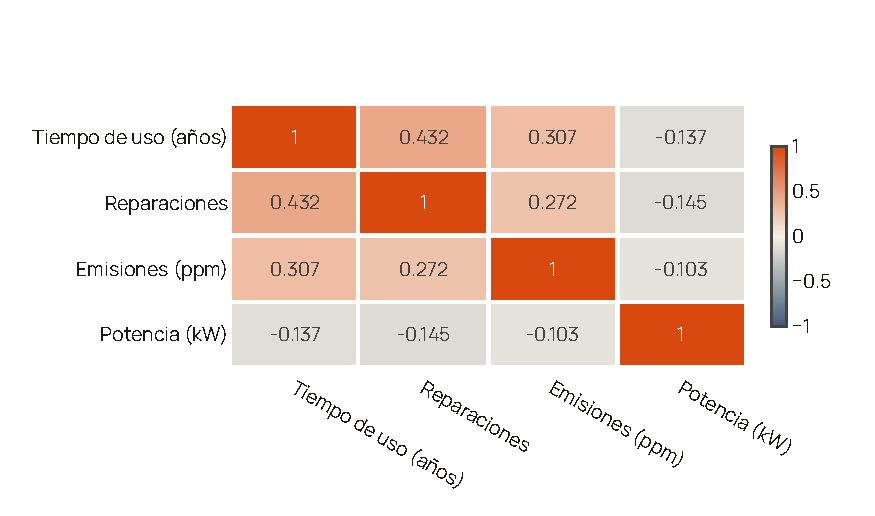
\includegraphics[width=\linewidth]{../figuras/f_corr.pdf}\end{minipage}\hfill
\begin{minipage}{0.54\linewidth}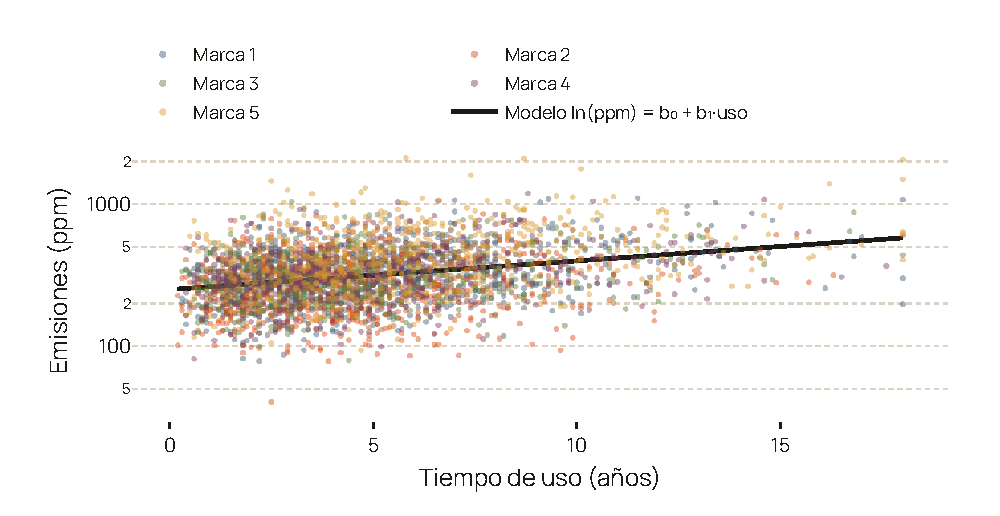
\includegraphics[width=\linewidth]{../figuras/f_disp_uso.pdf}\end{minipage}
\caption{Correlaciones de Pearson y modelo log-lineal de las emisiones frente al tiempo de uso.}\label{fig:rel}
\end{figure}
Las emisiones aumentan con el tiempo de uso ($r=\rUsoPpm$) y con las reparaciones ($r=\rRepPpm$), y la potencia baja
levemente con los años ($r=\rUsoPot$). El modelo $\ln(\widehat{ppm})=\regBcero+\regBuno\cdot\text{uso}$ indica que
\textbf{cada año de uso aumenta las emisiones un \regPct\,\%} en promedio. Las reparaciones de \mejor{} se ajustan a
una Poisson con $\hat\lambda=\poiLam$ ($EP=\poiEP$, $v=\poiV$, $P=\poiP$).

% =============================================================================
\section{Punto 2: comparación de dos equipos de procesamiento}\label{sec:p2}
% =============================================================================
Se generaron 60 tiempos (ms) por equipo con semilla 2026: en el escenario 1, $A\sim N(175,30)$ y
$B\sim N(170,50)$; en el escenario 2, $A\sim\Gamma(\alpha=1.2,\beta=150)$ y $B\sim\Gamma(0.95,190)$, con $\beta$ como
parámetro de escala ($E[X]=\alpha\beta$: 180 y 180.5 ms).

\subsection*{a) Histogramas, medidas descriptivas y pruebas de bondad de ajuste}
\figura[0.76]{f_hist4}{Histogramas ($k=6$ clases, $2^6>60$) con la densidad de la que se simularon los datos.}
\tabla[\footnotesize]{descr2}{Medidas descriptivas de los cuatro grupos (ms).}
Las medias muestrales del escenario 1 (\mediaA{} y \mediaB) se alejan de las teóricas más de lo que podría
parecer, lo que anticipa el literal b. En el escenario 2 la desviación es casi igual a la media (en la gamma,
$CV=1/\sqrt\alpha$) y la asimetría es fuerte (\asimC{} y \asimD).

\textbf{Ejemplo detallado (E1·A contra la normal).} Con $\hat\mu=\eaMu$ y $\hat\sigma=\eaS$ ($p=2$), las 6 clases
de igual ancho se reducen a \eaK{} al exigir $E_i\ge5$ (tabla~\ref{tab:chi_e1a}): $EP=\eaEP$, $v=\eaK-2-1=\eaV$,
$\chi^2_{(0.05,\eaV)}=\eaCrit$, $P=\eaP$. KS: $D=\eaD$, $P=\eaKsP$ (Lilliefors; el valor $P$ clásico \eaKsPc{} es
demasiado optimista). AD: $A^2=\eaAd$, $A^*=\eaAdMod<0.752$, $P=\eaAdP$. Las tres pruebas concluyen que \textbf{no
se rechaza la normalidad}.
\tabla[\footnotesize]{chi_e1a}{Prueba $\chi^2$ para E1·A contra $N(\eaMu,\ \eaS)$.}
\tabla[\footnotesize]{gof4}{Valores $P$ de las pruebas de ajuste a la normal y a la gamma (en rojo, $P<0.05$).}
\begin{figure}[H]\centering
\begin{minipage}{0.56\linewidth}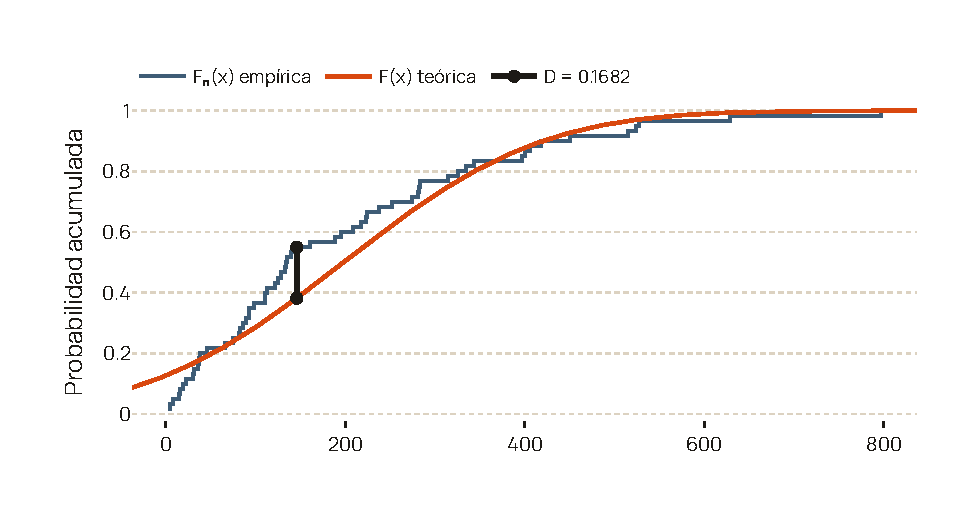
\includegraphics[width=\linewidth]{../figuras/f_ks_e2b.pdf}\end{minipage}\hfill
\begin{minipage}{0.42\linewidth}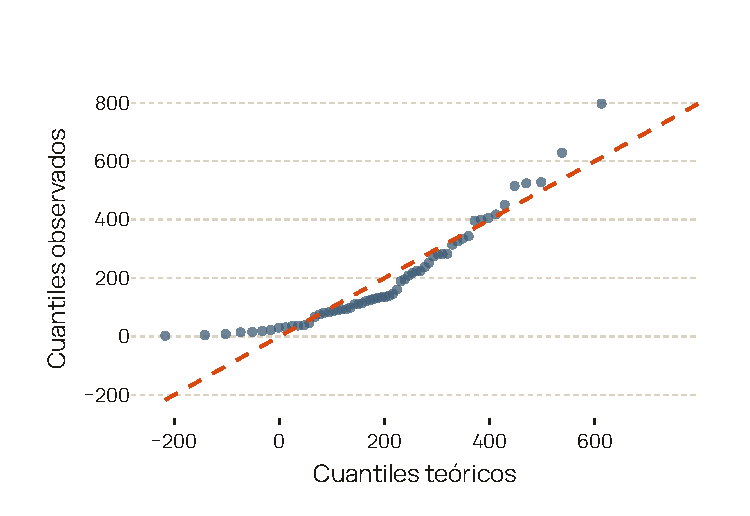
\includegraphics[width=\linewidth]{../figuras/f_qq_e2b.pdf}\end{minipage}
\caption{E2·B contra la normal: escalera empírica, curva normal ajustada y gráfico Q-Q.}\label{fig:e2b}
\end{figure}
\begin{lectura}
En el \textbf{escenario 1} ninguna prueba rechaza la normal, como se esperaba; tampoco se rechaza la gamma, porque
con $\alpha$ grande la gamma se parece a la normal y 60 datos no alcanzan para distinguirlas. En el
\textbf{escenario 2} KS ($D=\ebD$, $P\ebKsP$ para E2·B) y AD ($A^2=\ebAd$, $P\ebAdP$) rechazan la normal, mientras
que la gamma se acepta (E2·B: $\hat\alpha=\ebGalfa$, $\hat\beta=\ebGbeta$, AD $P=\ebGAdP$). La $\chi^2$ con clases
de igual ancho \emph{no puede decidir} en E2·A: la cola larga deja casi todos los datos en la primera clase y, al
agrupar, $v<1$. Ese es el argumento central para usar KS y AD: no agrupan y aprovechan cada dato. En el gráfico Q-Q
la curvatura en el extremo superior muestra la cola que la normal no puede reproducir.
\end{lectura}

\subsection*{b) Comparación de medias con $t$-Student y con la normal}
Para cada escenario se probó primero la igualdad de varianzas con $F$ (E1: $F=\feUno$, $P\fepUno$, distintas → $t$ de
\ttipoUno; E2: $F=\feDos$, $P=\fepDos$ → $t$ \ttipoDos). Luego, $H_0:\mu_A=\mu_B$:
\tabla[\footnotesize]{medias}{Pruebas de comparación entre los equipos A y B.}
\begin{lectura}
El estadístico es el \textbf{mismo número} con las dos distribuciones (E1: $t=Z=\ttUno$), porque ambas dividen la
diferencia de medias entre el mismo error estándar; cambia la distribución de referencia. La $t$ tiene colas más
pesadas y siempre da un valor $P$ algo mayor (E1: \tpUno{} frente a \zpUno): es la más \emph{conservadora}. Con 60
datos por grupo la diferencia es pequeña porque $t_{(\tglUno)}$ ya es casi normal, y por el TLC la $Z$ es válida
aunque los datos no sean normales. En el escenario 1 \textbf{se rechaza} $H_0$ (diferencia observada \difUno{} ms);
en el escenario 2 \textbf{no se rechaza} ($P=\tpDos$), coherente con medias teóricas casi iguales.
\end{lectura}

\subsection*{c) Prueba de Mann–Whitney}
\begin{figure}[H]\centering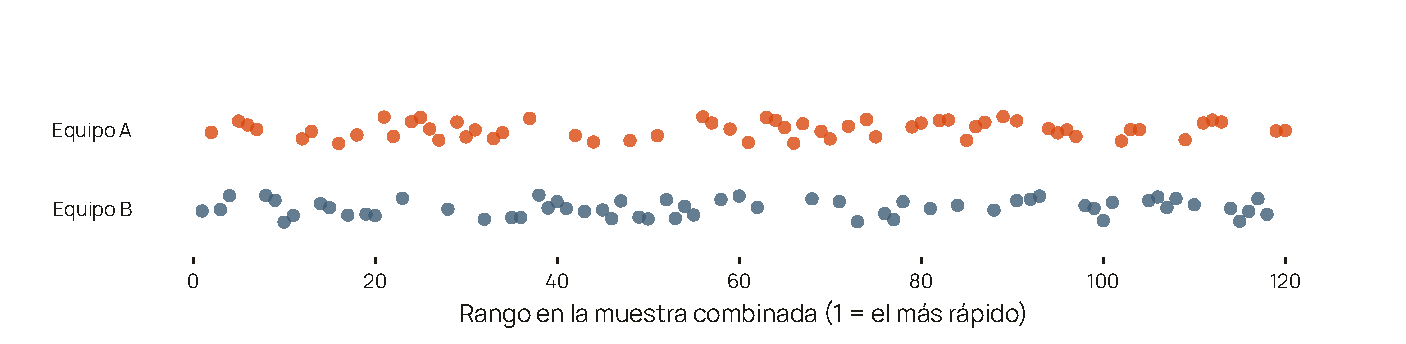
\includegraphics[width=0.8\linewidth]{../figuras/f_rangos_E2.pdf}
\caption{Rangos de los 120 tiempos del escenario 2 en la muestra combinada (1 = el más rápido).}\end{figure}
Escenario 2: $R_A=\mwRDos$, $U_A=\mwRDos-\tfrac{60\cdot61}{2}=\mwUDos$, $E[U]=\mwMuDos$, $\sigma_U=\mwSigDos$,
$Z=\mwZDos$, $P=\mwPDos$ (exacto: \mwPsDos). Escenario 1: $U_A=\mwUUno$, $Z=\mwZUno$, $P=\mwPUno$.
\begin{lectura}
En el \textbf{escenario 1}, con datos normales, Mann–Whitney y la $t$ llegan a la misma decisión
($P=\mwPUno$ y \tpUno): se rechaza $H_0$. En el \textbf{escenario 2} ninguna rechaza ($P=\mwPDos$ y \tpDos), pero
aquí Mann–Whitney es la prueba apropiada, porque los datos no son normales (literal a) y la media está dominada por
unos pocos tiempos muy largos. Su lectura es directa: tomado un trabajo al azar de cada equipo, el de A tarda más
en el $\mwSupDos\times100\,\%$ de los pares, prácticamente la mitad.
\end{lectura}

\subsection*{Valor agregado: ¿qué prueba es mejor? Un estudio de Monte Carlo}
Una sola muestra puede engañar. Se repitió 4000 veces el experimento completo y se contó cuántas veces cada prueba
rechaza $H_0$ (figura~\ref{fig:f_potencia_mc}).
\figura[0.7]{f_potencia_mc}{Porcentaje de rechazos en 4000 experimentos simulados por escenario.}
\begin{lectura}
Con dos poblaciones iguales (control) las tres pruebas rechazan cerca del 5\,\% (\mcTCtrl, \mcZCtrl{} y
\mcMwCtrl\,\%): están bien calibradas incluso con datos gamma. En el \textbf{escenario 1} la potencia apenas llega
al \mcTUno\,\%: con desviaciones de 30 y 50 ms, una diferencia real de 5 ms casi nunca se detecta con 60 datos, así
que \textbf{la muestra de este informe fue ``afortunada''}. En el \textbf{escenario 2}, $t$ y $Z$ rechazan
$\approx$5\,\%, porque las medias son iguales, mientras que Mann–Whitney rechaza algo más (\mcMwDos\,\%) porque
detecta la diferencia de \emph{forma}: $P(A>B)=\mcSupDos\neq0.5$.
\end{lectura}

% =============================================================================
\section{Punto 3: la Estadística en nuestras carreras, con datos reales}\label{sec:p3}
% =============================================================================
En \textbf{Ingeniería de Sistemas} la Estadística sostiene el aprendizaje automático (modelos, validación,
intervalos para métricas), las pruebas A/B de producto, la teoría de colas y la planeación de capacidad de
servidores, la confiabilidad y la detección de anomalías en seguridad, y las métricas de entrega de software
(DevOps), cuyo estudio más conocido es el de Forsgren, Humble y Kim \cite{accelerate}. En \textbf{Ingeniería
Industrial} es la base del control estadístico de procesos, el análisis de capacidad, Seis Sigma, el diseño de
experimentos, el muestreo de aceptación, el pronóstico de demanda y la simulación de sistemas productivos
\cite{montgomeryqc}. Como el grupo reúne estudiantes de ambas carreras, se desarrolló una aplicación de cada una.

\subsection{Ingeniería de Sistemas: el flujo de cambios de un proyecto de software}
\textbf{a) Problema.} Para dimensionar la integración continua (CI) y la capacidad de revisión de código, un equipo
necesita saber cuántos cambios llegan por día, de qué tamaño y si sirve el modelo de Poisson de la teoría de colas.
Se requieren la fecha, el tipo y el tamaño de cada cambio integrado, que se obtienen del historial de Git.

\textbf{b) Datos.} Se extrajo con \texttt{git log --first-parent --numstat} el historial de la rama principal de
Streamlit \cite{streamlit} entre el 1 de enero de 2024 y el 31 de diciembre de 2025. Tras quitar bots, publicaciones
de versión y commits sin cambios de texto quedaron \textbf{\nCommits{} commits} de \nAutores{} autores, cada uno
clasificado por palabras clave (corrección, funcionalidad, pruebas, refactorización, documentación,
mantenimiento), y se contaron los commits de cada uno de los \nDias{} días hábiles.

\textbf{c) Análisis.} \emph{c.1 Llegadas diarias.} $\bar x=\llMedia$ y $s^2=\llVar$: la varianza es
\llDisp{} veces la media, cuando la Poisson exige que sean iguales (\emph{sobredispersión}).
\figura[0.74]{f_llegadas}{Días hábiles según el número de commits, con lo esperado por cada modelo.}
\tabla[\footnotesize]{llegadas}{Prueba $\chi^2$ para las llegadas diarias.}
La Poisson se rechaza con contundencia ($EP=\poiCEP$, $v=\poiCV$, $P\poiCP$): hay \poiCeros{} días sin commits
cuando esperaba \poiCerosE, y muchos más días de alta actividad. La \textbf{binomial negativa} —una Poisson cuya tasa
cambia de un día a otro— sí se ajusta ($P=\bnP$). La diferencia es práctica: el percentil 95 con Poisson sería
\pnPoi{} commits/día; con la binomial negativa, \pnBn, y el real fue \pnReal.

\emph{c.2 Tamaño de los cambios.} Va de 1 a \tamMax{} líneas, con mediana \tamMed{} y media \tamMedia. Entre gamma,
Weibull, exponencial y lognormal, la \textbf{lognormal} tiene el menor AIC ($\hat\mu=\lgMu$, $\hat\sigma=\lgSig$ en
$\ln$ líneas). Con $n=\nCommits$ las pruebas la rechazan ($\chi^2$ equiprobable $P\lgChiP$; KS $D=\lgD$,
$P\lgKsP$; AD $P\lgAdP$): hay \lgPeq{} commits de 6 líneas o menos donde el modelo espera \lgPeqE. Con muestras tan
grandes cualquier desviación pequeña es significativa; el modelo describe bien el centro y la cola derecha.
\begin{figure}[H]\centering
\begin{minipage}{0.5\linewidth}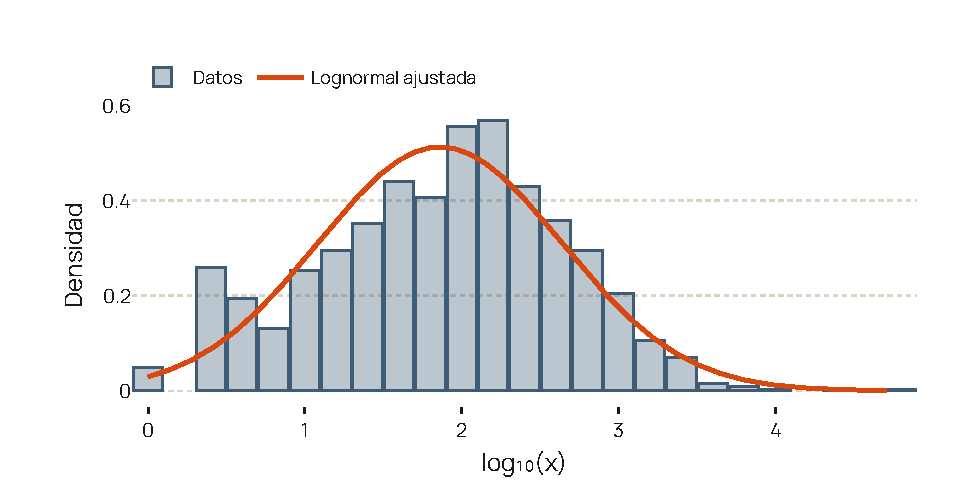
\includegraphics[width=\linewidth]{../figuras/f_lognormal.pdf}\end{minipage}\hfill
\begin{minipage}{0.48\linewidth}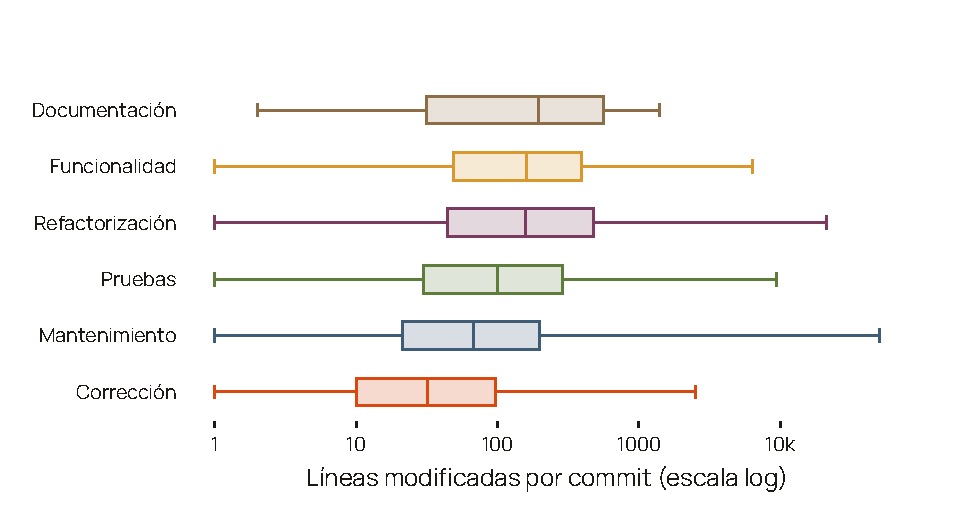
\includegraphics[width=\linewidth]{../figuras/f_cajas_tipo.pdf}\end{minipage}
\caption{Tamaño de los commits en escala logarítmica con la lognormal ajustada, y tamaño por tipo de cambio.}
\label{fig:tam}\end{figure}

\emph{c.3 Funcionalidades frente a correcciones.} Como los tamaños no son normales se usó Mann–Whitney: mediana de
\cfMf{} líneas en \cfNf{} funcionalidades y de \cfMc{} en \cfNc{} correcciones; $Z=\cfZ$, $P\cfP$. En el \cfSup\,\%
de los pares la funcionalidad es más grande (\rechaza).

\emph{c.4 Correlación y regresión.} El coeficiente de Pearson entre archivos y líneas modificadas es apenas
$r=\arR$, porque unos pocos commits gigantes dominan el cálculo; el de Spearman (rangos) es $\rho=\arRho$, y en escala
log-log $r=\arRlog$, con $\log_{10}\widehat{\text{líneas}}=\arBcero+\arBuno\log_{10}\text{archivos}$
($R^2=\arRdos$): duplicar los archivos multiplica las líneas por \arDoble. \emph{c.5} El \pcTot\,\% de los commits son
correcciones (IC 95\,\%: \pcLi–\pcLs\,\%); la proporción subió de \pcUno\,\% en 2024 a \pcDos\,\% en 2025
($Z=\pcZ$, $P=\pcP$).

\begin{lectura}
\textbf{d) Conclusiones y recomendaciones.} (1) No asumir Poisson para la llegada de trabajo humano: dimensionar la
CI con la binomial negativa (P95 = \pnBn{} commits/día). (2) El tamaño de un cambio es aproximadamente lognormal:
reportar medianas y percentiles, no promedios (la media, \tamMedia{} líneas, es más de tres veces la mediana). (3) Las funcionalidades son
\cfRazon{} veces más grandes que las correcciones: conviene dividirlas en cambios pequeños para revisarlas mejor.
(4) Para relacionar métricas de software, usar Spearman o transformar a logaritmos. (5) El aumento de las
correcciones sugiere reforzar las pruebas automatizadas.
\end{lectura}

\subsection{Ingeniería Industrial: ¿el proceso es capaz y está bajo control?}
\textbf{a) Problema.} (1) Los anillos de pistón de un motor deben medir $74.000\pm0.050$ mm: ¿el proceso está bajo
control, es capaz y cambió durante la vigilancia? (2) Una máquina llena latas de jugo y cada media hora se
inspeccionan 50: ¿los defectuosos siguen una binomial y mejoró el proceso tras ajustar la máquina? Se requieren
mediciones o conteos agrupados en muestras pequeñas a lo largo del tiempo.

\textbf{b) Datos.} Dos bases reales de Montgomery \cite{montgomeryqc}, distribuidas en el paquete \texttt{qcc} de R
\cite{qcc}: 40 muestras de 5 diámetros (las 25 primeras, fase I) y 54 muestras de 50 latas (las 30 primeras, fase I;
las muestras 15 y 23 tienen causas asignables documentadas y se excluyen).

\textbf{c) Análisis.} Con la fase I, $\bar{\bar x}=\xbb$ y $\bar R=\rb$, de modo que $LSC_{\bar x}=\lscx$,
$LIC_{\bar x}=\licx$ y $LSC_R=\lscr$.
\figura[0.84]{f_carta_x}{Carta $\bar X$ de los anillos de pistón. En rojo, los puntos fuera de control.}
Los diámetros de la fase I son normales ($\chi^2$: $P=\anChiP$; KS: $P=\anKsP$; AD: $P=\anAdP$), lo que valida la
carta y los índices: $C_p=\anCp$ y $C_{pk}=\anCpk$, ambos mayores que 1.33. El proceso es \textbf{capaz} (se
esperan \anPpm{} piezas defectuosas por millón) y está centrado (IC 95\,\% de $\mu$: [\anIcLi, \anIcLs] mm;
$t=\anTn$, $P=\anTnP$ frente a 74). En la fase II, las muestras 37, 38 y 39 salen sobre el límite: la media se
desplazó de \faMuno{} a \faMdos{} mm, \faMicras{} micras (IC 95\,\%: \faIcLi{} a \faIcLs{} micras), lo que la prueba
$t$ confirma ($t=\faT$, $P\faP$), mientras que la variabilidad no cambió de forma clara ($F=\faF$, $P=\faFP$).
\figura[0.84]{f_carta_p}{Carta $p$ de las latas de jugo; las muestras 15 y 23 (causas asignables) se excluyen del cálculo.}
\begin{minipage}{0.48\linewidth}
Con $\bar p=\juPbar$, los límites son $LSC=\juLsc$ y $LIC=\juLic$. El número de latas defectuosas por muestra se
ajusta a una Binomial$(50,\ \juBp)$: $EP=\juEP$, $v=\juK-1-1=\juV$, crítico \juCrit, $P=\juP$ (\norechaza).
Tras ajustar la máquina la fracción bajó a \juPdos; la prueba de dos proporciones da $Z=\juZ$, $P\juPz$: una mejora
real de \juIcLi{} a \juIcLs{} puntos porcentuales.
\end{minipage}\hfill
\begin{minipage}{0.48\linewidth}\centering{\footnotesize\sans\begin{tabular}{lrrrr}
\toprule
\textbf{Clase} & \textbf{$O_i$} & \textbf{$P_i$} & \textbf{$E_i=nP_i$} & \textbf{$(O_i-E_i)^2/E_i$} \\ \midrule
0–8 & 9 & 0.22338 & 6.255 & 1.2049 \\
9 y 10 & 6 & 0.25552 & 7.154 & 0.1863 \\
11 y 12 & 4 & 0.25443 & 7.124 & 1.3699 \\
13–50 & 9 & 0.26667 & 7.467 & 0.3148 \\
\bottomrule
\end{tabular}}\end{minipage}

\begin{lectura}
\textbf{d) Conclusiones y recomendaciones.} (1) El proceso de anillos es capaz y estuvo bajo control en la fase I.
(2) En la fase II la media subió \faMicras{} micras: aunque todavía no hay piezas fuera de especificación, debe
buscarse la causa antes de que el corrimiento crezca. (3) El ajuste de la llenadora redujo los defectuosos de
\juPbar{} a \juPdos, pero un 11\,\% sigue siendo alto: se recomienda un análisis de Pareto de las causas y
recalcular la carta $p$. (4) Las cartas dependen de los modelos normal y binomial: las pruebas de ajuste no son un
trámite, sino lo que hace válidos sus límites.
\end{lectura}

% =============================================================================
\section*{Conclusiones}
\addcontentsline{toc}{section}{Conclusiones}
\begin{enumerate}
\item \textbf{Hornos.} \mejor{} es la marca de mejor desempeño global: la que menos contamina y menos se daña. Su
potencia media está entre \muLi{} y \muLs{} kW (centrada en 2.70) y su cumplimiento de emisiones es consistente con
la afirmación del fabricante (80\,\%). Marca 3 es la más uniforme en potencia: su varianza es significativamente
menor que la de Marca 4.
\item \textbf{Equipos A y B.} Las pruebas $t$ y $Z$ dan el mismo estadístico y valores $P$ casi iguales con $n=60$; la
$t$ es ligeramente más conservadora. Con datos gamma, Mann–Whitney es la prueba adecuada. El estudio de Monte Carlo
mostró que con 60 datos la potencia para detectar 5 ms de diferencia es de solo \mcTUno\,\%.
\item \textbf{Las tres pruebas de ajuste se complementan.} $\chi^2$ es la única para variables discretas; KS y AD
aprovechan cada dato y, con los valores $P$ corregidos por simulación, son las más potentes. AD destaca en las
colas, que es donde suelen estar los problemas de ingeniería.
\item \textbf{Datos reales.} La llegada de trabajo a un repositorio no es Poisson sino binomial negativa, y el tamaño
de los cambios es aproximadamente lognormal; el proceso de anillos es capaz pero se desplazó en la vigilancia, y el
ajuste de la llenadora mejoró la calidad de forma significativa.
\item \textbf{Valor de la herramienta.} La aplicación en Python replica exactamente el ejemplo de la guía
($EP=\astonEP$, $P=\astonP$), permite repetir cada análisis con otros datos y hace explícitos los supuestos que
el Excel no muestra.
\end{enumerate}

% =============================================================================
\begin{thebibliography}{99}\small
\addcontentsline{toc}{section}{Referencias}
\bibitem{guia} H. Fernández C., ``Pruebas de bondad de ajuste'', guía del curso Estadística para Ingeniería,
Facultad de Ingenierías, Universidad de Medellín, 2026.
\bibitem{walpole} R. E. Walpole, R. H. Myers, S. L. Myers y K. Ye, \emph{Probabilidad y estadística para
ingeniería y ciencias}, 9.ª ed. México: Pearson, 2012.
\bibitem{montgomery} D. C. Montgomery y G. C. Runger, \emph{Applied Statistics and Probability for Engineers},
7.ª ed. Hoboken, NJ: Wiley, 2018.
\bibitem{montgomeryqc} D. C. Montgomery, \emph{Introduction to Statistical Quality Control}, 8.ª ed. Hoboken, NJ:
Wiley, 2019.
\bibitem{kolmogorov} A. N. Kolmogorov, ``Sulla determinazione empirica di una legge di distribuzione'',
\emph{Giornale dell'Istituto Italiano degli Attuari}, vol. 4, pp. 83--91, 1933.
\bibitem{smirnov} N. Smirnov, ``Table for estimating the goodness of fit of empirical distributions'', \emph{Ann.
Math. Statist.}, vol. 19, no. 2, pp. 279--281, 1948.
\bibitem{ad1952} T. W. Anderson y D. A. Darling, ``Asymptotic theory of certain `goodness of fit' criteria based on
stochastic processes'', \emph{Ann. Math. Statist.}, vol. 23, no. 2, pp. 193--212, 1952.
\bibitem{ad1954} T. W. Anderson y D. A. Darling, ``A test of goodness of fit'', \emph{J. Amer. Statist. Assoc.},
vol. 49, no. 268, pp. 765--769, 1954.
\bibitem{stephens} M. A. Stephens, ``EDF statistics for goodness of fit and some comparisons'', \emph{J. Amer.
Statist. Assoc.}, vol. 69, no. 347, pp. 730--737, 1974.
\bibitem{lilliefors} H. W. Lilliefors, ``On the Kolmogorov--Smirnov test for normality with mean and variance
unknown'', \emph{J. Amer. Statist. Assoc.}, vol. 62, no. 318, pp. 399--402, 1967.
\bibitem{razali} N. M. Razali y Y. B. Wah, ``Power comparisons of Shapiro--Wilk, Kolmogorov--Smirnov, Lilliefors
and Anderson--Darling tests'', \emph{J. Stat. Model. Anal.}, vol. 2, no. 1, pp. 21--33, 2011.
\bibitem{mannwhitney} H. B. Mann y D. R. Whitney, ``On a test of whether one of two random variables is
stochastically larger than the other'', \emph{Ann. Math. Statist.}, vol. 18, no. 1, pp. 50--60, 1947.
\bibitem{wilcoxon} F. Wilcoxon, ``Individual comparisons by ranking methods'', \emph{Biometrics Bulletin}, vol. 1,
no. 6, pp. 80--83, 1945.
\bibitem{accelerate} N. Forsgren, J. Humble y G. Kim, \emph{Accelerate: The Science of Lean Software and DevOps}.
Portland, OR: IT Revolution Press, 2018.
\bibitem{streamlit} Streamlit Inc., ``streamlit/streamlit'', repositorio de GitHub. [En línea]. Disponible en:
\url{https://github.com/streamlit/streamlit}. Consultado: 30 oct. 2026.
\bibitem{qcc} L. Scrucca, ``qcc: an R package for quality control charting and statistical process control'',
\emph{R News}, vol. 4, no. 1, pp. 11--17, 2004.
\bibitem{scipy} P. Virtanen \emph{et al.}, ``SciPy 1.0: fundamental algorithms for scientific computing in
Python'', \emph{Nature Methods}, vol. 17, pp. 261--272, 2020.
\end{thebibliography}

% =============================================================================
\newpage
\appendix
\renewcommand{\thesection}{\Alph{section}}
\section{La herramienta en Python}\label{anx:app}
La aplicación se ejecuta con \texttt{python -m streamlit run app.py} y se organiza en un índice lateral de ocho
páginas: portada con el mapa de temas del curso, los tres puntos del proyecto, el laboratorio de datos propios, la
teoría de las pruebas de ajuste y el taller de la guía. El nivel de significancia, la confianza, la semilla y el
número de repeticiones de Monte Carlo se cambian en la barra lateral y todo se recalcula.
\begin{figure}[H]\centering
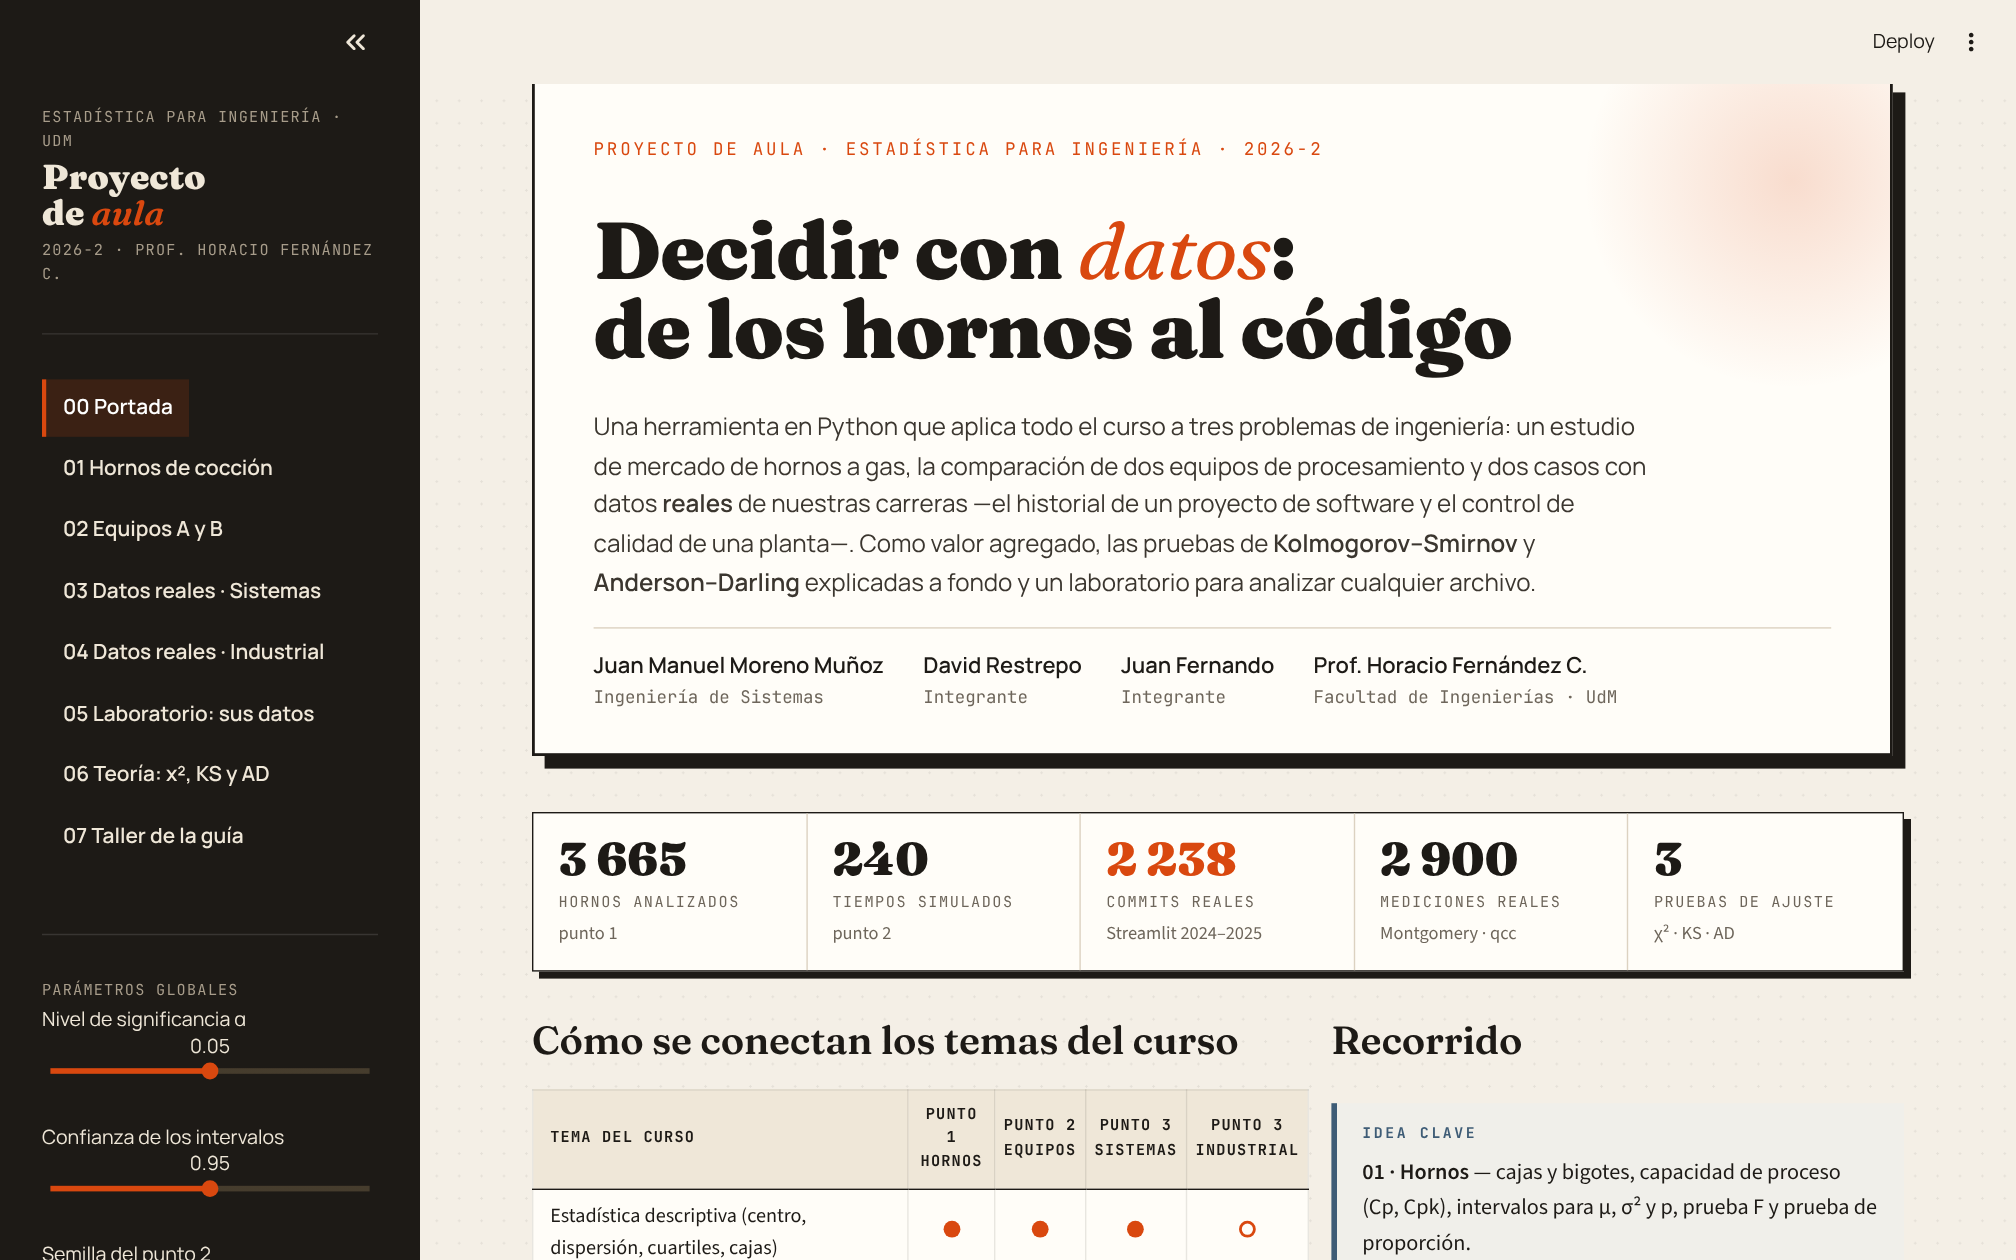
\includegraphics[width=0.49\linewidth]{../figuras/app_portada.png}\hfill
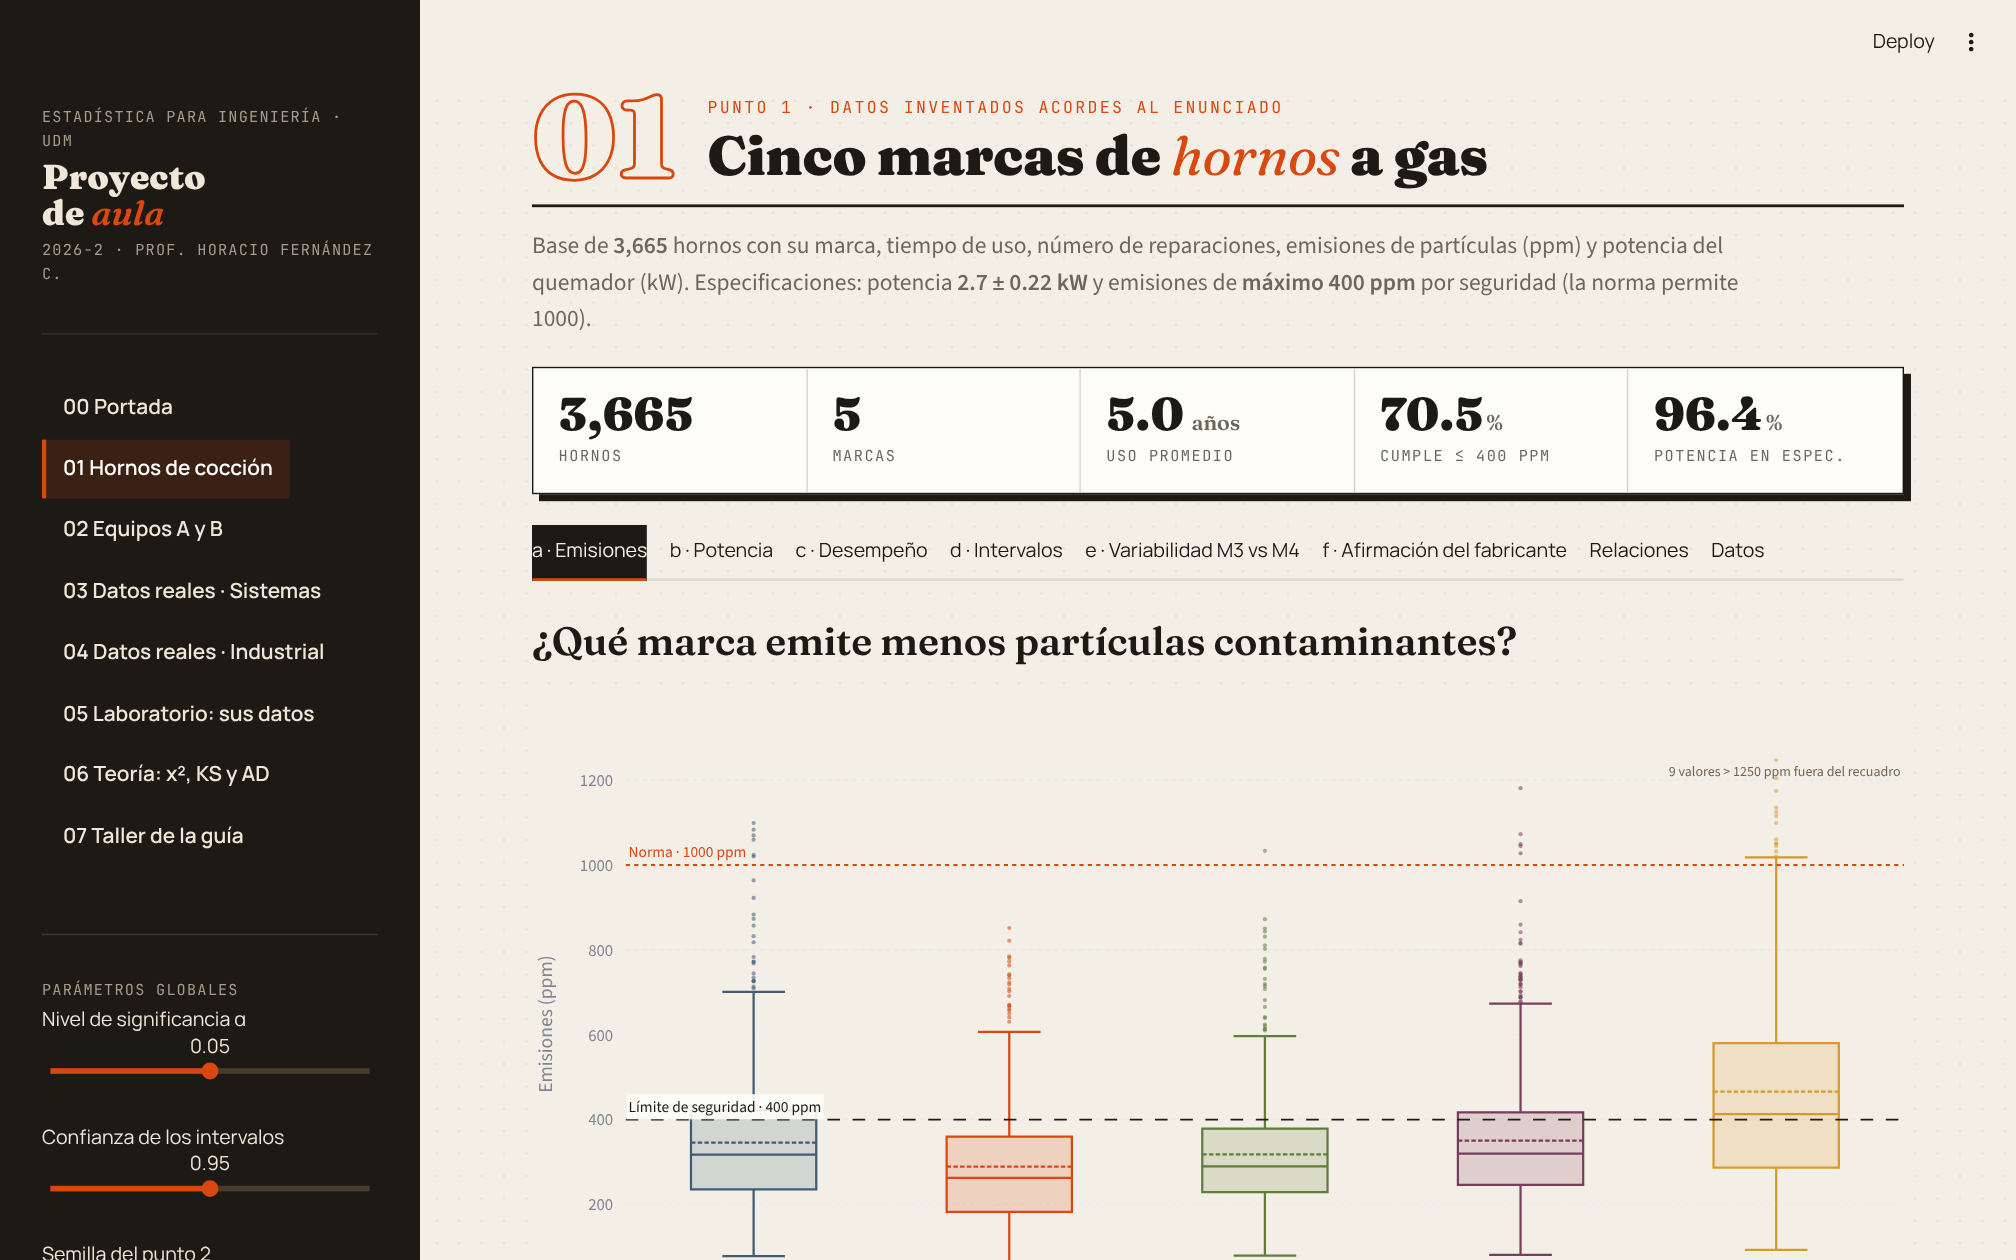
\includegraphics[width=0.49\linewidth]{../figuras/app_hornos.png}\\[4pt]
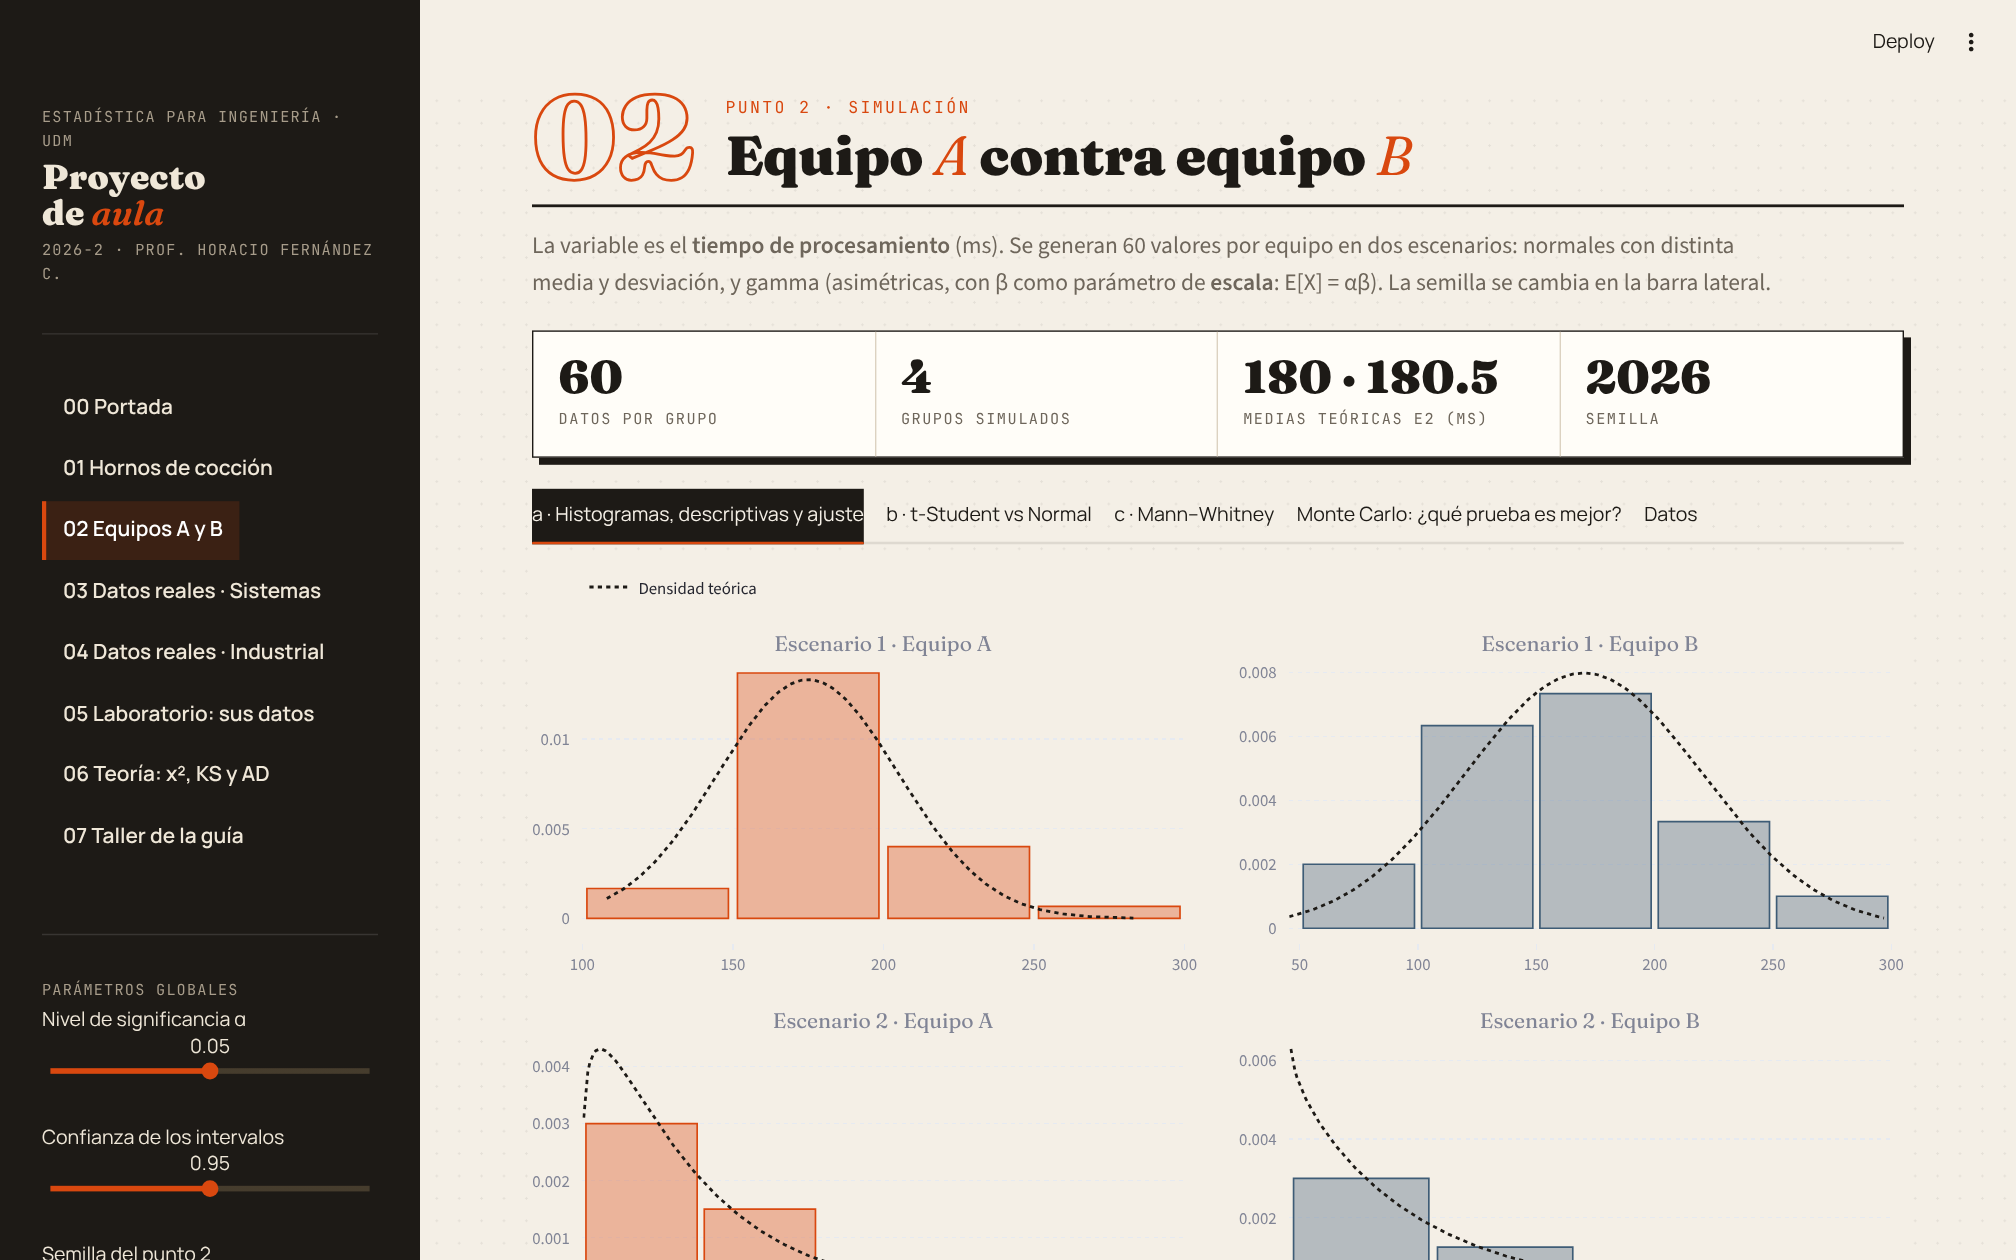
\includegraphics[width=0.49\linewidth]{../figuras/app_equipos.png}\hfill
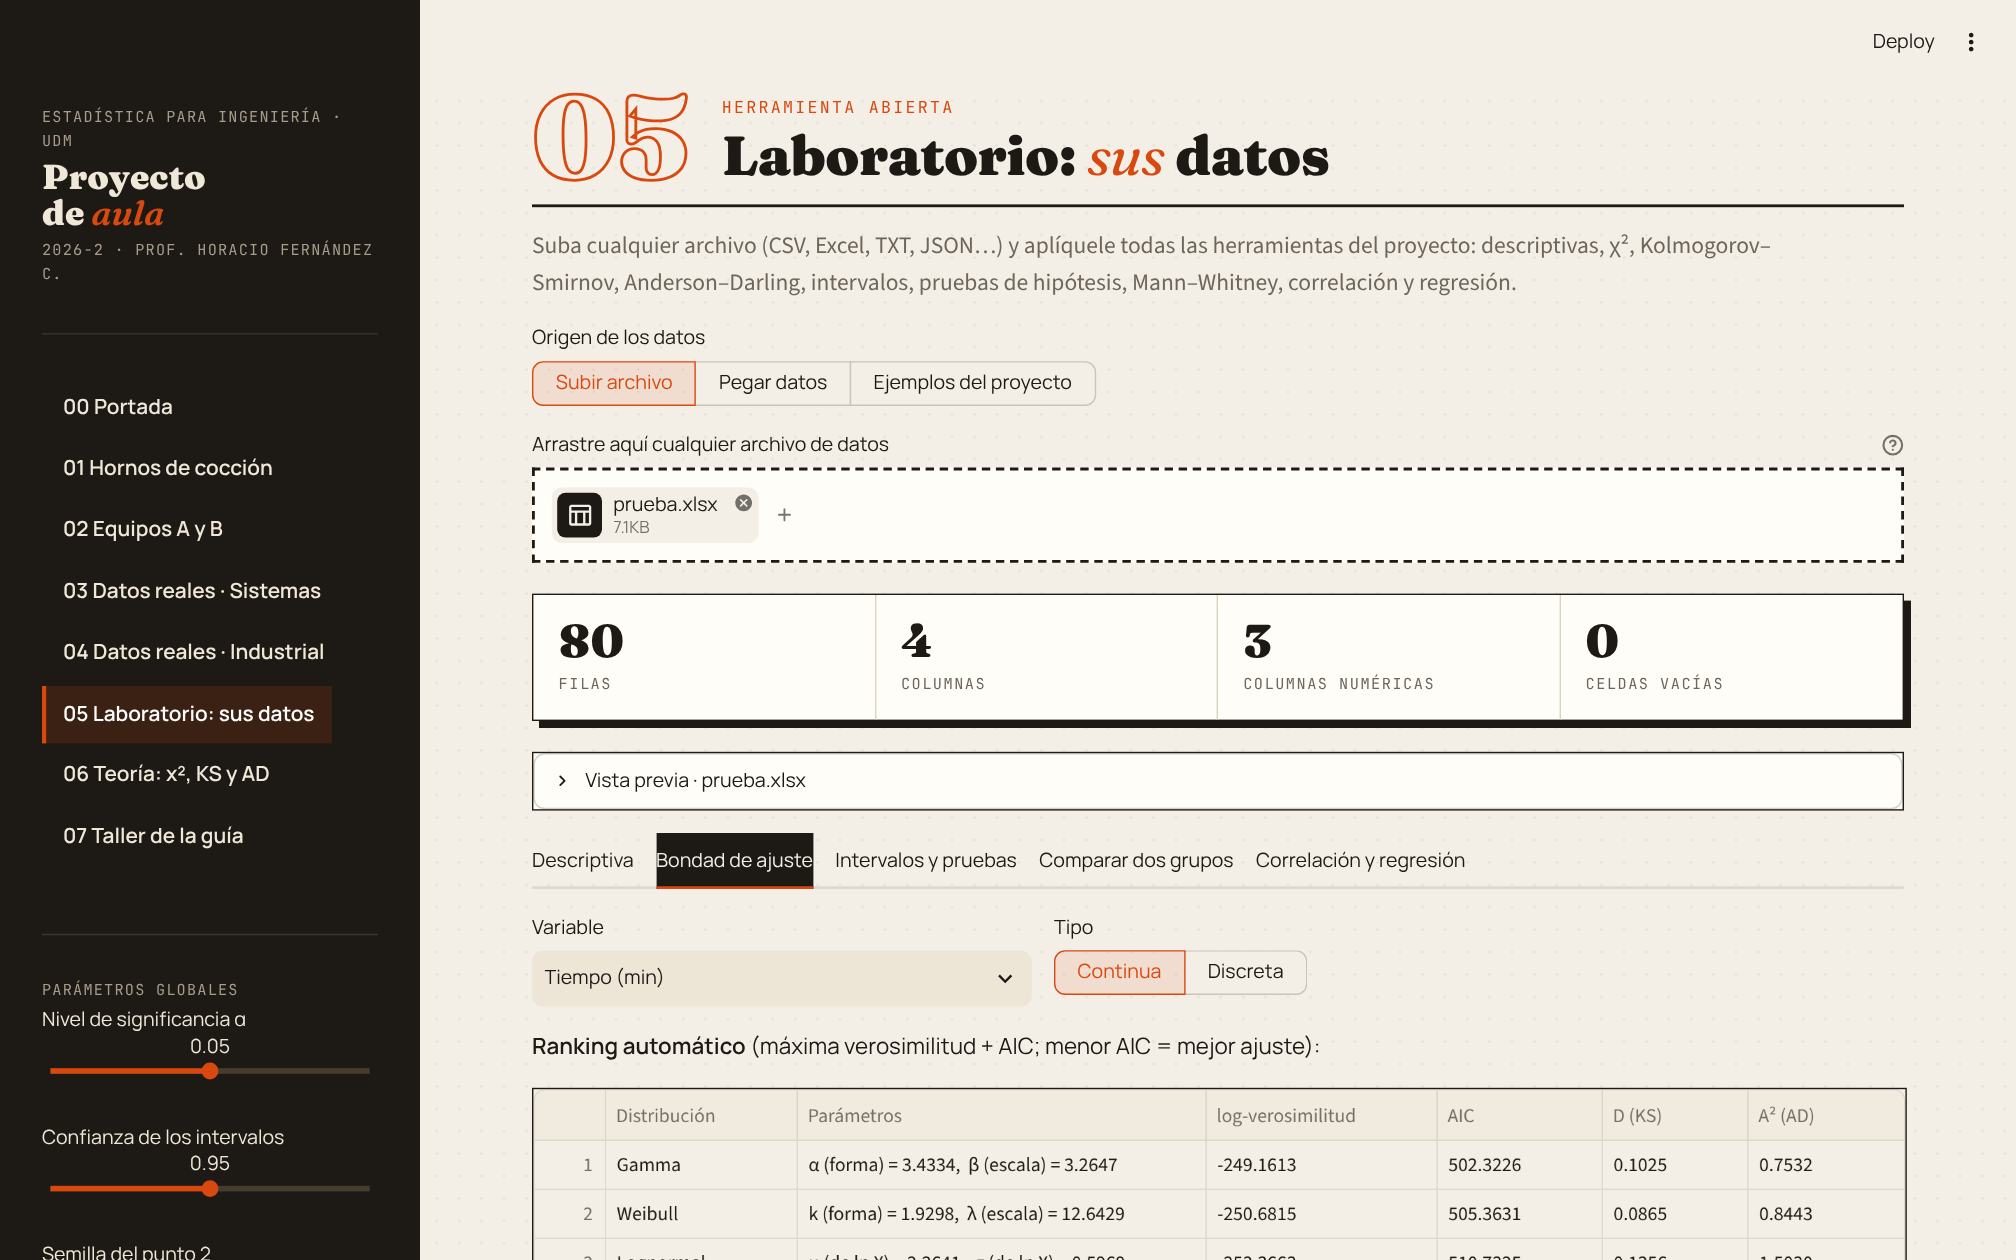
\includegraphics[width=0.49\linewidth]{../figuras/app_laboratorio.png}
\caption{Portada, punto 1, punto 2 y laboratorio con un archivo de Excel cargado.}\end{figure}
\textbf{Laboratorio.} Acepta CSV, TXT, TSV (separados por coma, punto y coma, tabulador o espacios, con decimales
de punto o de coma), Excel (\texttt{.xlsx}, \texttt{.xls}, \texttt{.ods}), JSON y Parquet; también se pueden pegar
datos copiados de Excel. Para la columna elegida ofrece medidas descriptivas, un ranking automático de
distribuciones por AIC, las tres pruebas de ajuste (o $\chi^2$ para Poisson, binomial y binomial negativa si la
variable es discreta), intervalos y pruebas sobre la media y la proporción, comparación de dos grupos ($F$, Levene,
$t$, $Z$, Mann–Whitney) y correlación y regresión.

\textbf{Estructura del repositorio.} \texttt{app.py} (interfaz); \texttt{src/} con el motor estadístico
(\texttt{bondad.py}, \texttt{inferencia.py}, \texttt{descriptiva.py}, \texttt{montecarlo.py}, \texttt{hornos.py},
\texttt{aplicaciones.py}, \texttt{taller.py}) separado de las páginas (\texttt{src/paginas/}); \texttt{scripts/}
para regenerar los datos y todos los números y figuras del informe; \texttt{data/} con las bases; \texttt{excel/} y
\texttt{r/} con los cálculos equivalentes. Las pruebas se apoyan en NumPy, SciPy \cite{scipy}, pandas y Plotly.

\section{Taller de la guía resuelto}
El motor de la aplicación se validó con el ejemplo de la guía: reproduce $EP=6.38393$, $v=7$ y $P=0.4957$ con las
mismas probabilidades redondeadas a cinco decimales. La tabla~\ref{tab:taller} resume el ejemplo y los seis
ejercicios. \emph{Nota:} la última línea del ejemplo en la guía dice que $H_0$ ``debe ser rechazada''; como
$P=0.4957>0.05$, la conclusión correcta es que \emph{no} se rechaza, como indica el párrafo anterior de la misma guía.
\tabla[\scriptsize]{taller}{Ejemplo y ejercicios de la guía de bondad de ajuste.}
\begin{itemize}
\item \textbf{Ej. 1.} Se rechaza la Normal(2.5, 0.4) al 5\,\% por poco: en la clase $x>2.95$ hay 22 baterías y se
esperaban 13; las baterías duran más de lo propuesto. Con $\alpha=0.01$ no se rechazaría.
\item \textbf{Ej. 2.} No se rechaza la normalidad de la rentabilidad diaria ($p=2$ parámetros estimados).
\item \textbf{Ej. 3.} No se rechaza la Poisson para las averías semanales con $\alpha=0.01$.
\item \textbf{Ej. 4.} Se rechaza la Poisson: las llegadas son más regulares de lo que predice (varianza menor que la
media), con exceso de minutos con 2 y 3 vehículos.
\item \textbf{Ej. 5.} No se rechaza la Poisson(0.5) para los defectos del componente AH233.
\item \textbf{Ej. 6.} Se rechaza la binomial: hay demasiados días con 0 o 1 acciones vendidas; las tres acciones de
un mismo día no son independientes porque todas dependen del mercado de ese día.
\end{itemize}

\section{Reproducibilidad: Python, Excel y R}
\begin{table}[H]\centering\small\caption{Equivalencia de los cálculos principales.}
\begin{tabularx}{\linewidth}{lXX}\toprule
\textbf{Cálculo} & \textbf{Excel} & \textbf{R}\\\midrule
$t_{\alpha/2,n-1}$, $\chi^2_{a,v}$, $z_{\alpha/2}$ & \texttt{T.INV.2T}, \texttt{CHISQ.INV.RT}, \texttt{NORM.S.INV} &
\texttt{qt}, \texttt{qchisq}, \texttt{qnorm}\\
Probabilidades $P_i$ & \texttt{NORM.DIST}, \texttt{POISSON.DIST}, \texttt{BINOM.DIST}, \texttt{GAMMA.DIST} &
\texttt{pnorm}, \texttt{dpois}, \texttt{dbinom}, \texttt{pgamma}\\
Valor $P$ de $\chi^2$ & \texttt{CHISQ.DIST.RT(EP; v)} & \texttt{pchisq(EP, v, lower.tail = FALSE)}\\
Prueba $F$ y $t$ & \texttt{F.TEST}, \texttt{T.TEST} & \texttt{var.test}, \texttt{t.test}\\
KS y AD & estadísticos con fórmulas por fila & \texttt{ks.test}, \texttt{nortest::ad.test}, \texttt{nortest::lillie.test}\\
Mann–Whitney & rangos con \texttt{RANK.AVG} & \texttt{wilcox.test}\\\bottomrule
\end{tabularx}\end{table}
Los datos simulados se generan en Python con la semilla 2026 y se guardan en \texttt{data/}; Excel y R leen esos
mismos archivos, de modo que los tres entornos trabajan sobre los mismos números. Para regenerar todo:
\begin{center}\texttt{python scripts/generar\_datos.py}\quad·\quad\texttt{python scripts/generar\_informe.py}\quad·\quad
\texttt{python scripts/generar\_excel.py}\end{center}
\end{document}
